\subsection{Fatos estilizados da economia norte-americana}\label{FatosEUA}

%Desse modo, a literatura do supermultiplicador é um contraponto ao \textit{trade-off} apontado por \textcite{solow_importance_1995} uma vez que são os gastos autônomos que lideram o crescimento no longo prazo.

Dentre os componentes da demanda agregada, o investimento das firmas figura entre os mais investigados pela literatura.
Dentre as razões pelas quais tal gasto é tão estudado, destacam-se sua elevada volatilidade e considerável participação no PIB.
O investimento residencial, por sua vez, não possui uma participação tão grande na renda (gráfico \ref{FigAutonomos}), mas --- ao contrário do que indicaria a intuição --- é mais volátil que o PIB e que o investimento das firmas (gráfico \ref{FigVolatilidade}). 
O principal objetivo desta seção é destacar que a pouca atenção dada ao investimento residencial não é compatível com seu grau de importância para a economia norte-americana e que esta relevância não se restringe à crise imobiliária recente.
%Adicionalmente, procura-se mostrar que, ao contrário de \textcite{grebler_capital_1956}, tal relevância não só não se apequenou como tem se amplificado  \cites{fiebiger_semi-autonomous_2018}{karwowski_financialisation_2019}{walther_forty_2019}.
Em paralelo, serão apresentados alguns fatos estilizados que irão contextualizar as simulações do capítulo \ref{CapModelo}.



%%%%%%%%%%%%%%%%%%%%%%%%%%%%% PEQUENA PARTICIPAÇÃO NO PIB %%%%%%%%%%%%%%%%%%%%%%%%%%%

\begin{figure}[H]
	\centering
	\caption{Participação dos gastos autônomos no PIB dos EUA (1979-2019)}
	\label{FigAutonomos}
	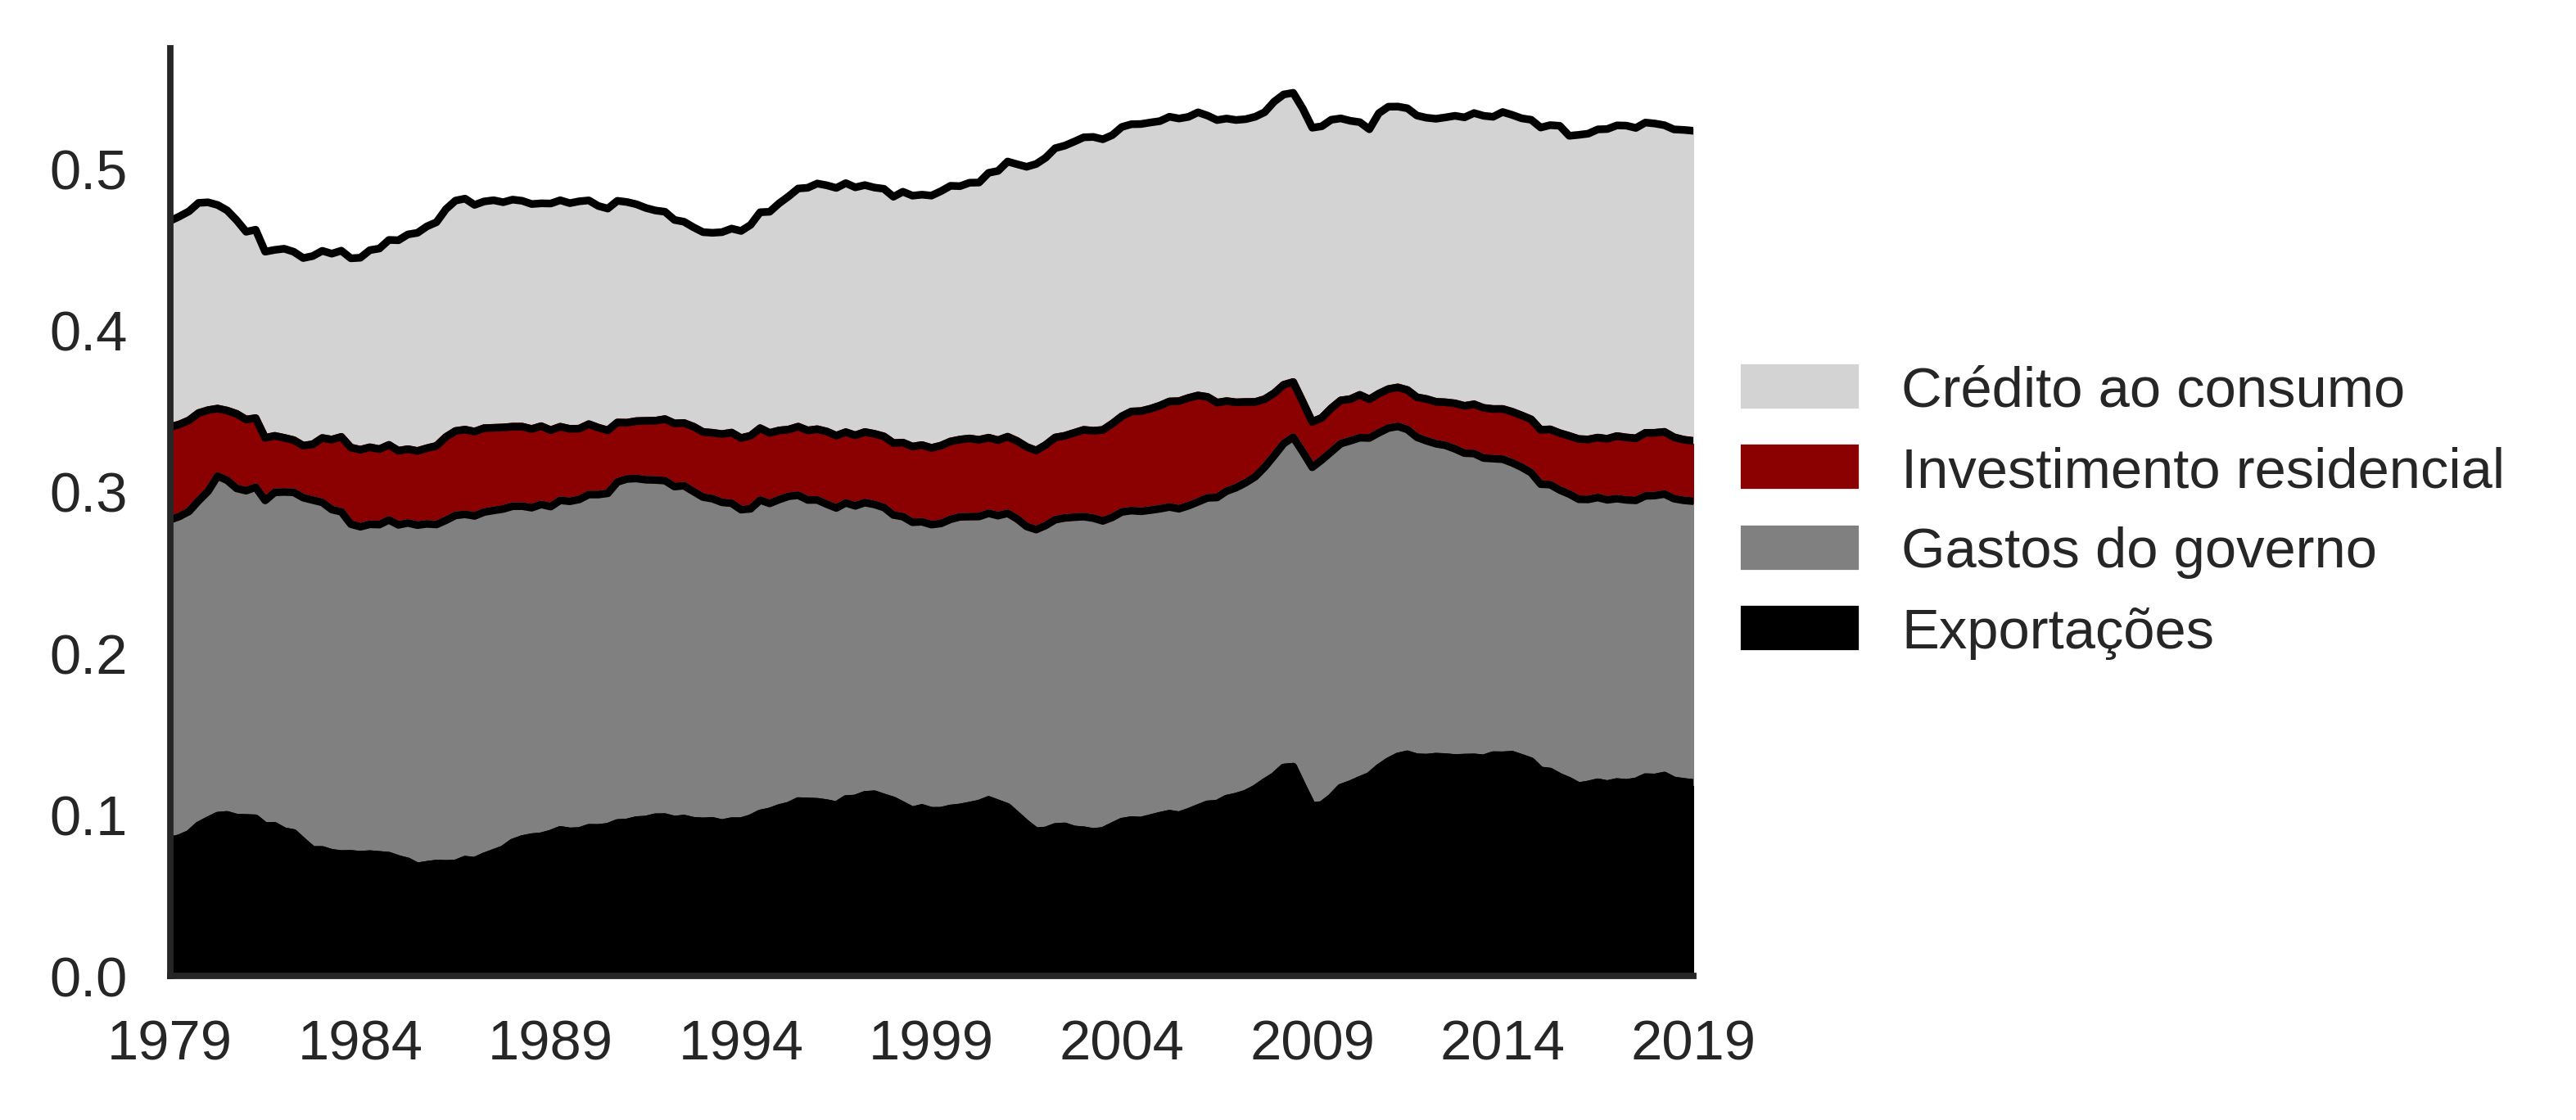
\includegraphics[width=\textwidth]{../../Dados/Fatos_Estilizados/figs/Gastos_autonomos.png}
	\caption*{\textbf{Fonte:} U.S. Bureau of Economic Analisys, elaboração própria}
\end{figure}


\begin{figure}[H]
	\centering
	\caption{Distribuição de taxas de crescimento selecionadas (1947-2007 e 2009-2019)}
	\label{FigVolatilidade}
	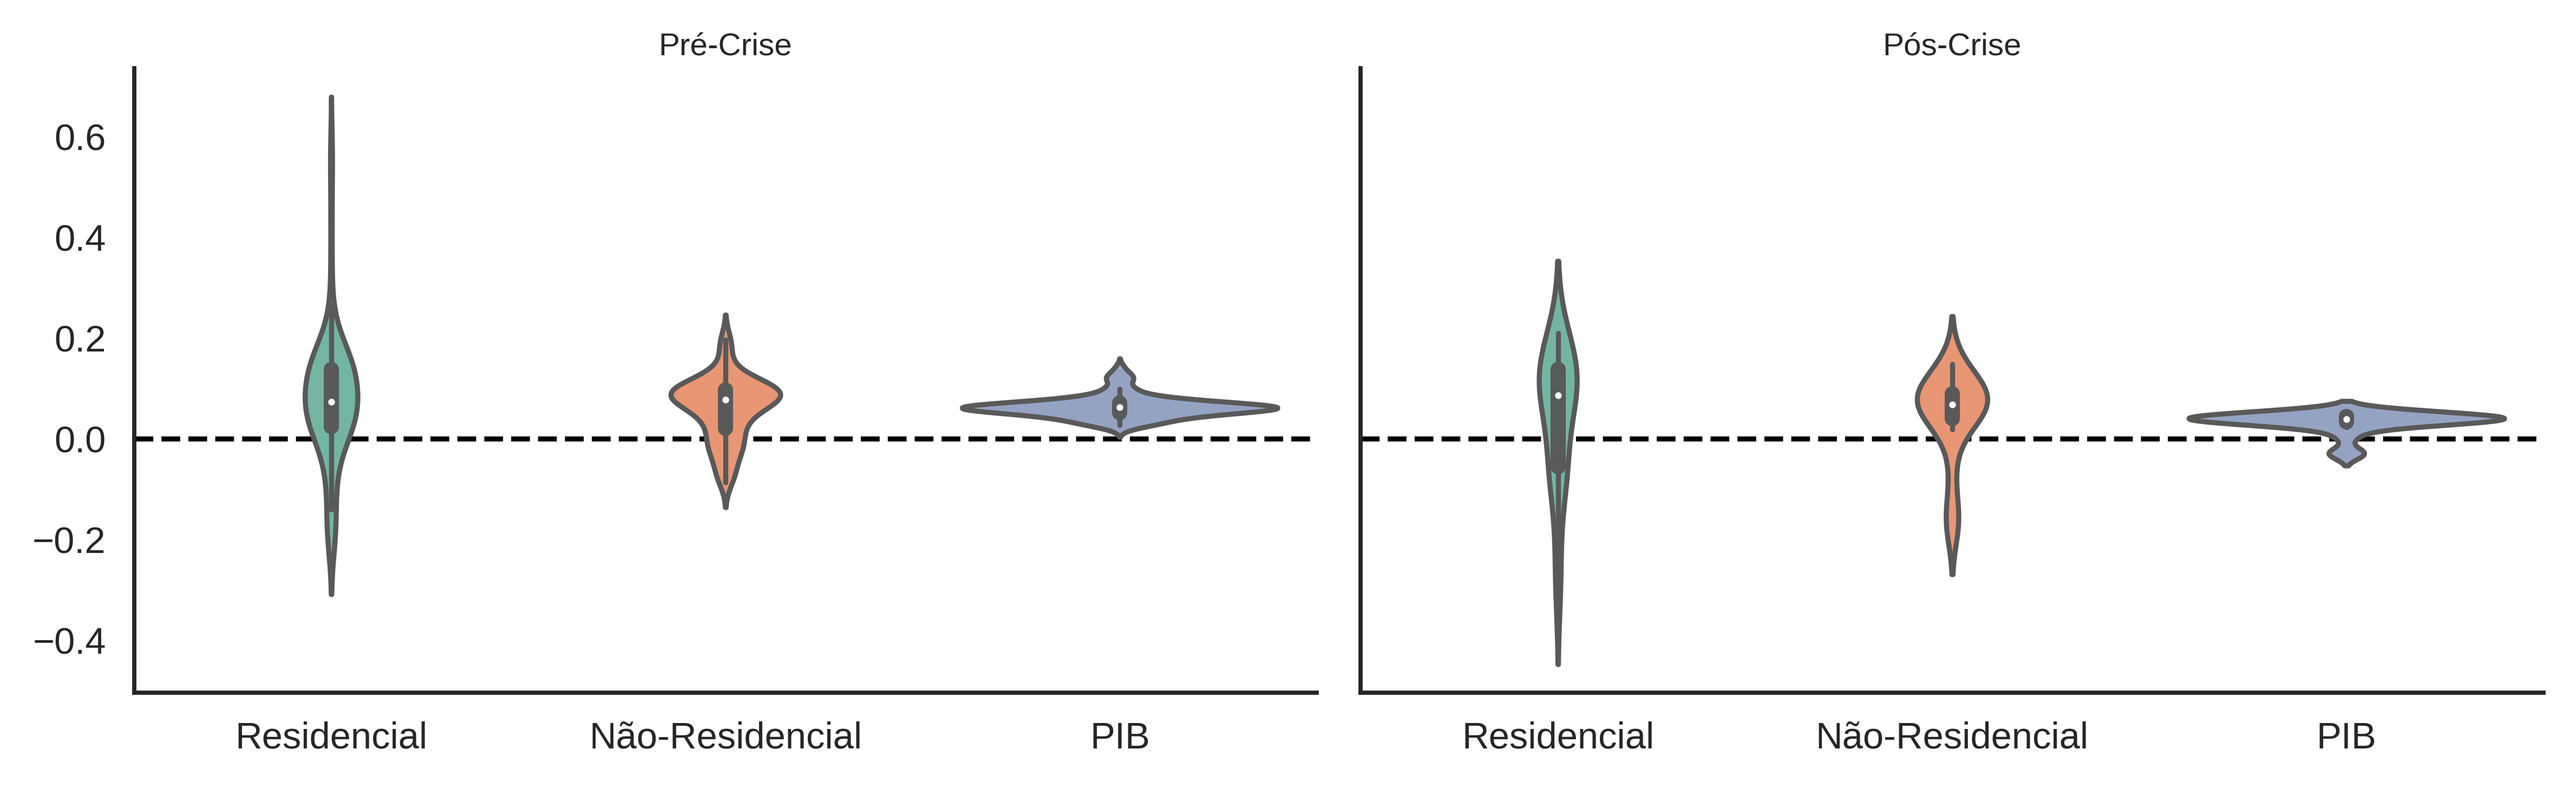
\includegraphics[width=\textwidth]{../../Dados/Fatos_Estilizados/figs/Volatilidade.png}
	\caption*{\textbf{Fonte:} U.S. Bureau of Economic Analisys, elaboração própria}
\end{figure}

Neste ponto, cabe mencionar o ineditismo de \textcite{green_follow_1997} e \textcite{leamer_housing_2007} --- e revisitado em \textcite{leamer_housing_2015} e por \textcite{fiebiger_trend_2017} --- ao lançar luz sobre a importância do investimento residencial na determinação dos ciclos econômicos antes mesmo da crise dos \textit{subprimes}. 
Ao avaliar o caso norte-americano, \textcite{green_follow_1997} conclui que o
investimento residencial lidera --- mais que o investimento das firmas --- o ciclo econômico, mas, ao mesmo tempo, reconhece que isso não implica o estabelecimento de uma relação causal. Na tentativa de compreender tais resultados, afirma:

\begin{citacao}
	
	[P]erhaps residential investiment, like stock prices and interest rates, is a good predictor of GDP because it is a series that reflects \textbf{foward looking behavior}. Presumably households will not increase their expenditures on housing unless they expect to prosper in the future. Building a house is a natural mechanism for doing this. Thus, the series can do a good job of predicting GDP without necessarily causing GDP.
	\cite[p.~267, grifos adicionados]{green_follow_1997}
\end{citacao}
Apesar de dar atenção para um gasto não criador de capacidade, o argumento de \textcite{green_follow_1997} se difere das conclusões do supermultiplicador sraffiano uma vez que não são estes gastos que lideram o crescimento.
\textcite{leamer_housing_2007}, por sua vez, avança em direção a relação de causalidade entre este gasto e o PIB. Grosso modo, afirma que a construção de novos imóveis implica maior consumo de bens duráveis e, portanto, trata-se de um ciclo decorrente do \textit{volume} e não do preço dos imóveis. 

Uma forma de visualizar a importância do investimento residencial para o ciclo econômico na economia estadunidense é por meio do gráfico \ref{FigIh_u} em que cada um dos painéis apresenta um ciclo iniciado no primeiro trimestre de crescimento positivo após a recessão e se estende até o fim da recessão seguinte\footnote{
	Raciocínio semelhante pode ser encontrado em \textcite{fiebiger_semi-autonomous_2018} em que, diferentemente do presente trabalho, não é incluído consumo financiado por crédito.}. 
No eixo vertical, observa-se a participação desse gasto no PIB, enquanto no eixo horizontal, o grau de utilização da capacidade como uma \textit{proxy} para o ciclo econômico. Exceto para o período 1991-2001, a recuperação (aumento da utilização da capacidade) é caracterizada por uma taxa de crescimento do investimento residencial maior que o crescimento da economia, resultando em maior participação desse gasto no PIB. Considerando que as firmas seguem o princípio do ajuste do estoque de capital, ampliam a taxa de acumulação de modo a ajustar o grau de utilização para o grau normal. O aumento da taxa de crescimento do investimento das firmas e de outros gastos reduz a participação do investimento residencial no PIB. A maturação do investimento das firmas, por sua vez, redunda em menor utilização da capacidade produtiva\footnote{
	Complementarmente, os trabalhos de \textcite{fiebiger_semi-autonomous_2018} e \textcite{fiebiger_trend_2017} também reportam o investimento residencial como determinante do comportamento cíclico e adicionam o consumo financiado por crédito a essa dinâmica. Além disso, apresentam uma similaridade com \textcite{dejuan_hidden_2017} e \textcite{teixeira_crescimento_2015} para os quais a instabilidade econômica está associada à instabilidade (ao menos de alguns) gastos autônomos e não do investimento das firmas, que segue o princípio do ajuste do estoque de capital.}. 
Com o deflagrar da crise, o grau de utilização cai e o ciclo se encerra no fim da recessão e se reinicia --- no painel seguinte --- com a economia sendo puxada pelo investimento residencial.



\begin{figure}[H]
	\centering
	\caption{Relação entre taxa de investimento residencial e grau de utilização por recessão}
	\label{FigIh_u}
	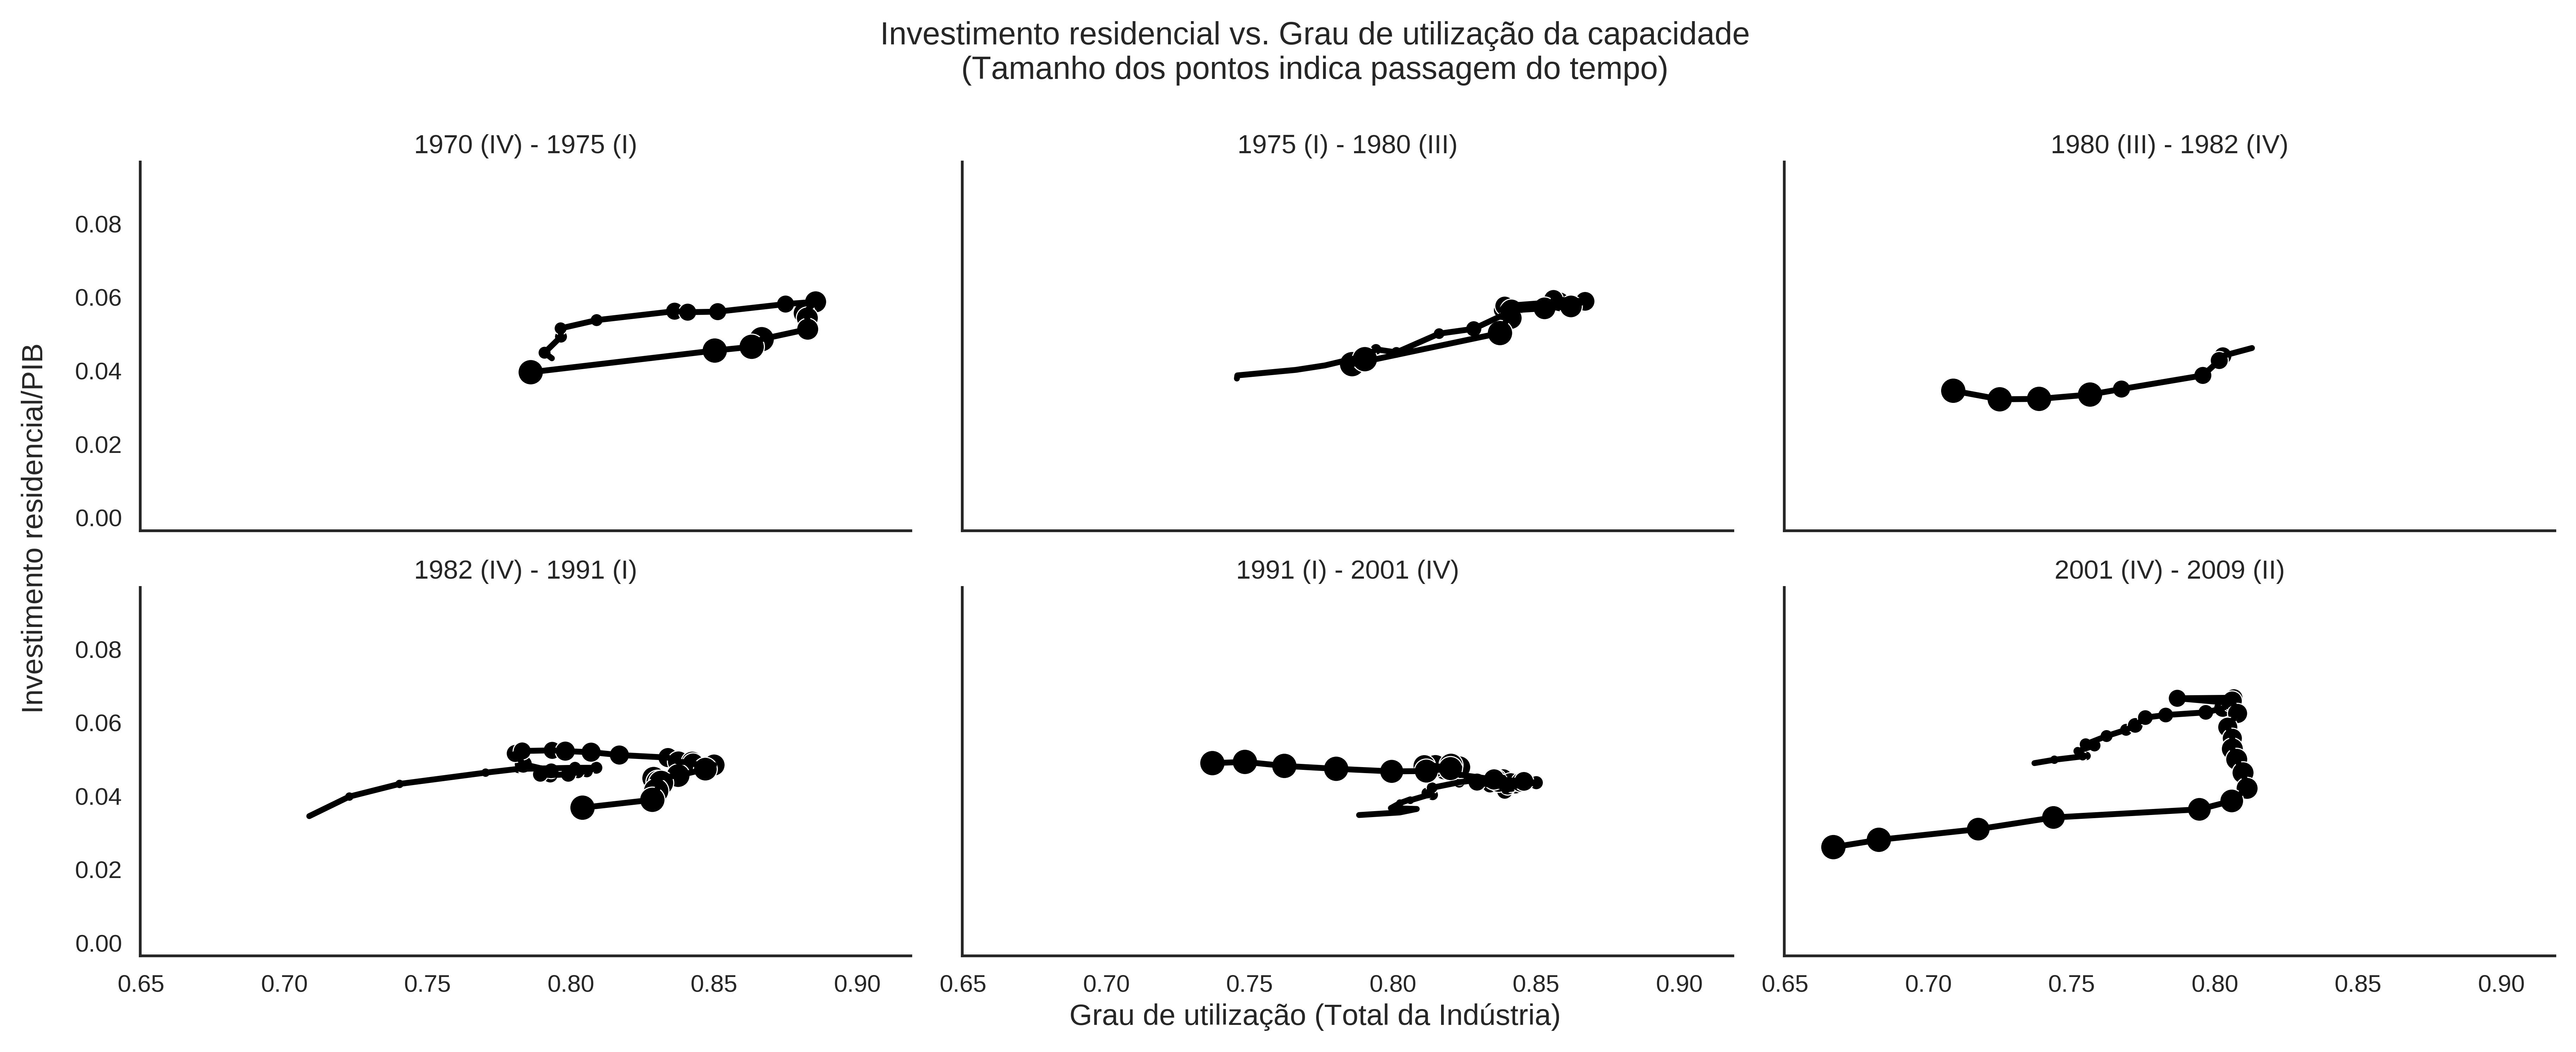
\includegraphics[width=\textwidth]{../../Dados/Fatos_Estilizados/figs/Ciclo_Ih_u.png}
	\caption*{\textbf{Fonte:} Elaboração própria}
\end{figure}

%%%%%%%%%%%%%%%%%%%%%%% GRÁFICO RELÓGIO DURÁVEIS %%%%%%%%%%%%%%%%%%

Como mencionado anteriormente, além de liderar o ciclo econômico, o investimento residencial também está relacionado com o consumo de bens duráveis.
O gráfico \ref{FigInvesto_Duraveis} ilustra tal associação em que é feita a mesma periodização das crises dos painéis anteriores com a diferença de que o eixo horizontal apresenta a participação do consumo de bens duráveis na renda. 
Diferentemente do gráfico anterior, este não apresenta um comportamento cíclico tão demarcado ao longo do período que antecedeu a Grande Recessão. Apesar disso, é possível visualizar que a economia desacelera na medida que estes gastos decrescem (conjuntamente) enquanto o crescimento conjunto destes gastos na recuperação não é tão evidente em todos os ciclos (destaque para o ciclo de 1975 a 1980).
De toda maneira, tais gráficos denotam uma especifidade do ciclo econômico norte-americano que pode ser resumida nos seguintes termos: ``\textit{[f]irst homes, then cars, and last business equipment}'' \cite[p.~8]{leamer_housing_2007}.

\begin{figure}[H]
	\centering
	\caption{Relação entre taxa de investimento residencial e grau de utilização por recessão}
	\label{FigInvesto_Duraveis}
	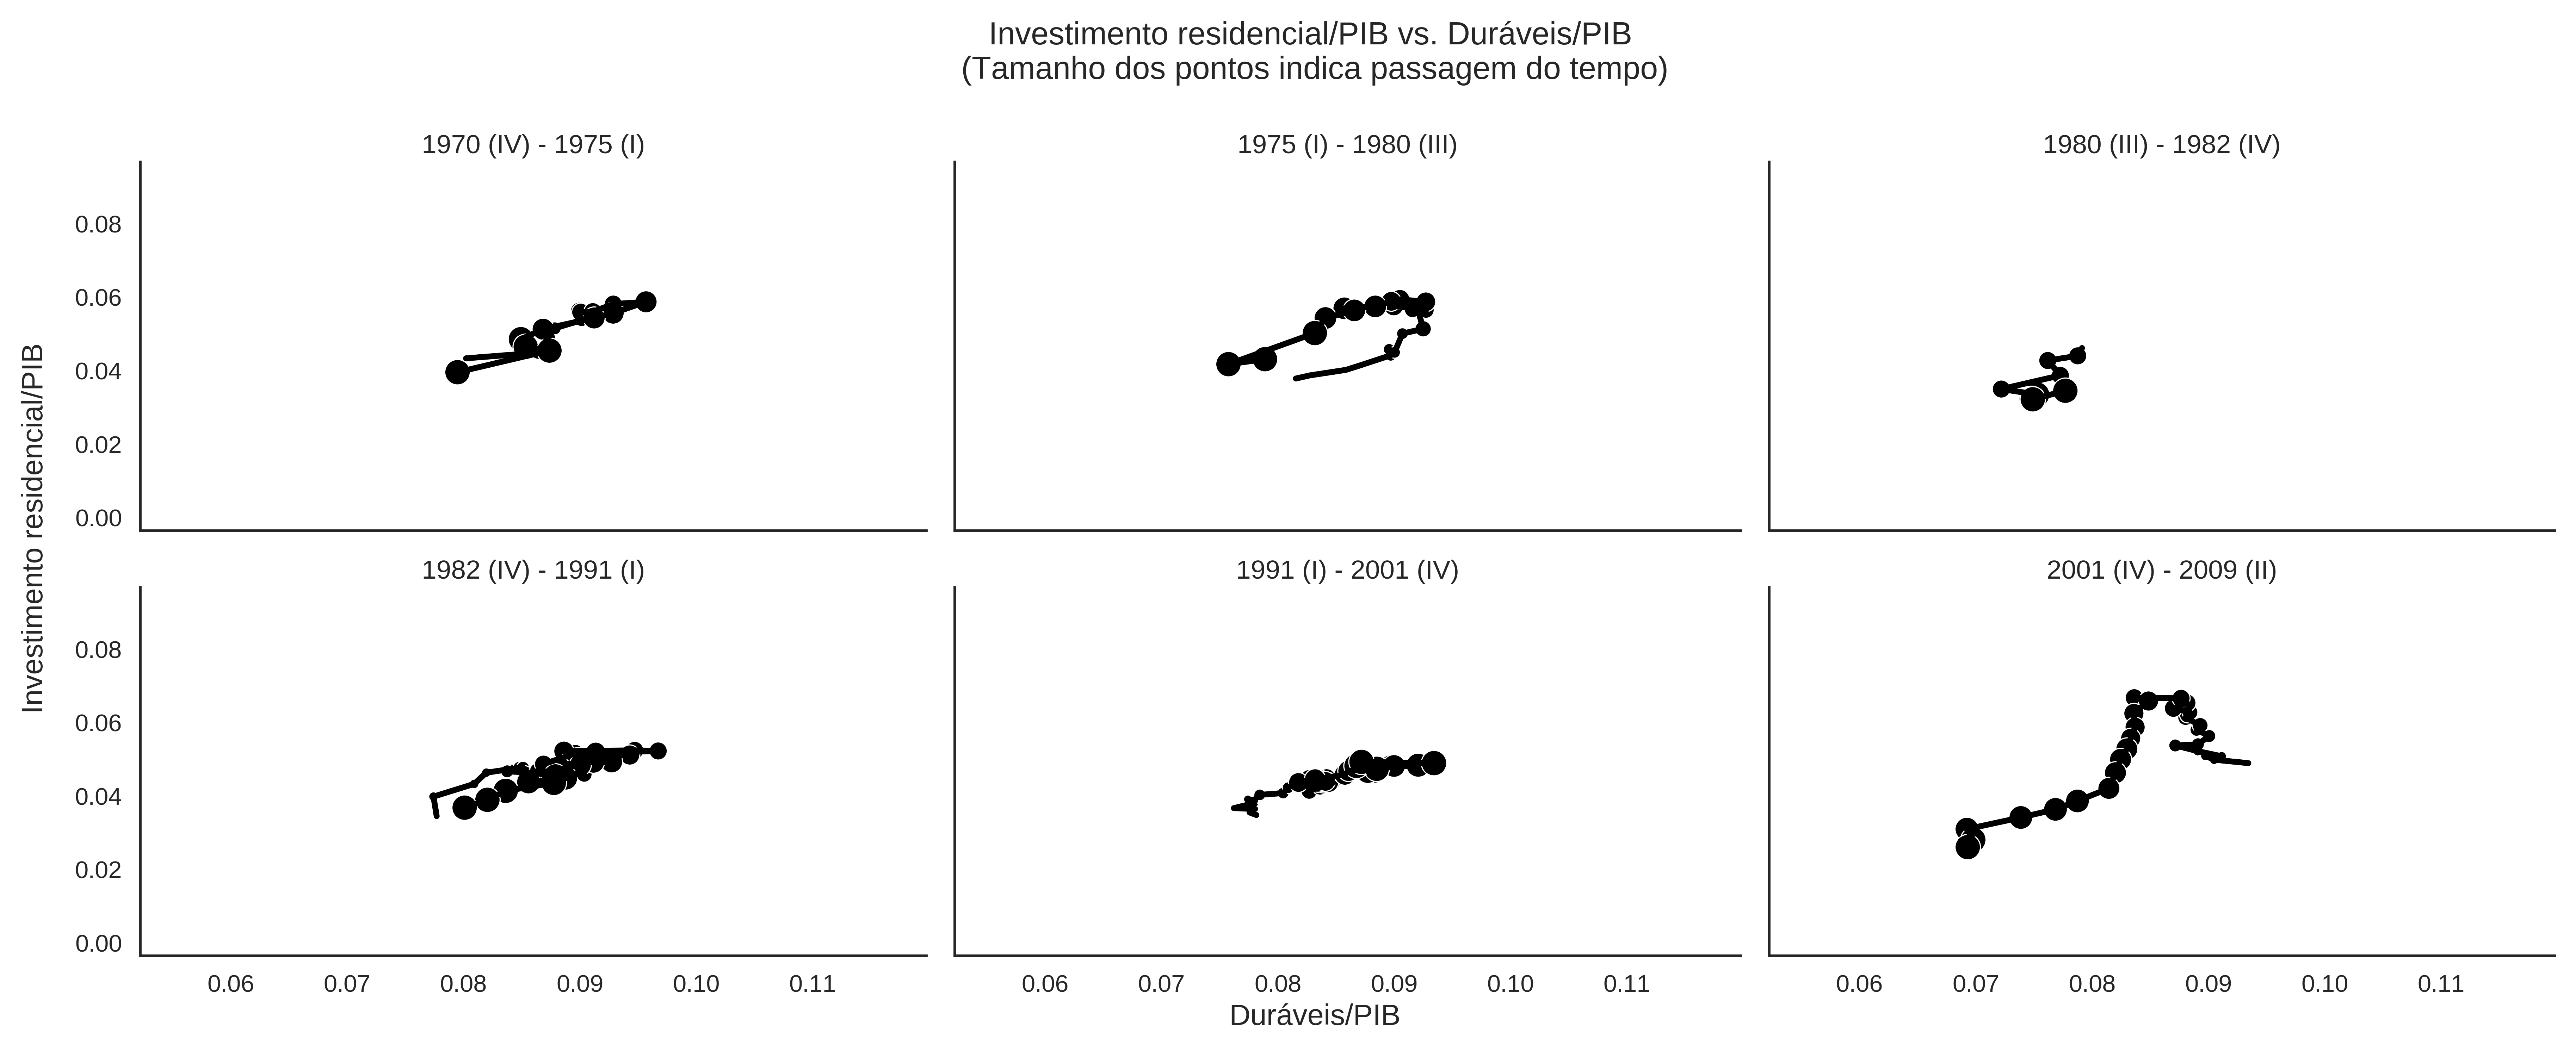
\includegraphics[width=\textwidth]{../../Dados/Fatos_Estilizados/figs/Ciclo_Ih_Duraveis.png}
	\caption*{\textbf{Fonte:} Elaboração própria}
\end{figure}

Desse modo, conclui-se que o investimento residencial ajuda a compreender os ciclos econômicos americanos.
Resta realçar como a compreensão deste componente da demanda permite esclarecer tanto as recessões quanto as retomadas. Esta dinâmica pode ser visualizada nos gráficos \ref{FigCriseNorm} e \ref{FigRecuperacaoNorm} em que são apresentadas as taxas de crescimento do produto, consumo financiado por crédito, investimento residencial e não-residencial (normalizadas para manter a comparatibilidade)\footnote{
	Nestes gráficos, as taxas de crescimento são normalizadas para facilitar a comparatibilidade uma vez que é mantida uma mesma escala uma vez que o investimento residencial apresenta uma taxa de crescimento mais ampla em relação às demais. 
	Dito isso, adotou-se o procedimento convencional de normalização, qual seja, calculou-se o desvio da taxa de crescimento em relação à média pelo seu respectivo desvio-padrão.
	Sendo assim, se esta taxa de crescimento normalizada for negativa, não implica necessariamente em uma taxa de crescimento negativa, mas sim abaixo da média.
} nos trimestres que antecedem e sucedem as recessões/recuperações. 
Destaca-se a redução da taxa de crescimento do investimento residencial nos trimestres que antecedem as recessões enquanto passa a ter taxas positivas antes das recuperações, liderando-as.
Em outras palavras, observa-se que o investimento residencial possui uma taxa de crescimento (a taxas crescentes) positiva nos trimestres que antecedem a recuperação enquanto o investimento das firmas só apresenta tal comportamento adiante. Portanto, esse gráfico ilustra tanto a capacidade do investimento residencial liderar o ciclo quanto a indução do investimento criador de capacidade produtiva.


\begin{figure}[H]
	\centering
	\caption{Taxas de crescimento 4 trimestres antes e depois do início da  \textbf{recessão} (normalizadas para manter a comparatibilidade)}
	\label{FigCriseNorm}
	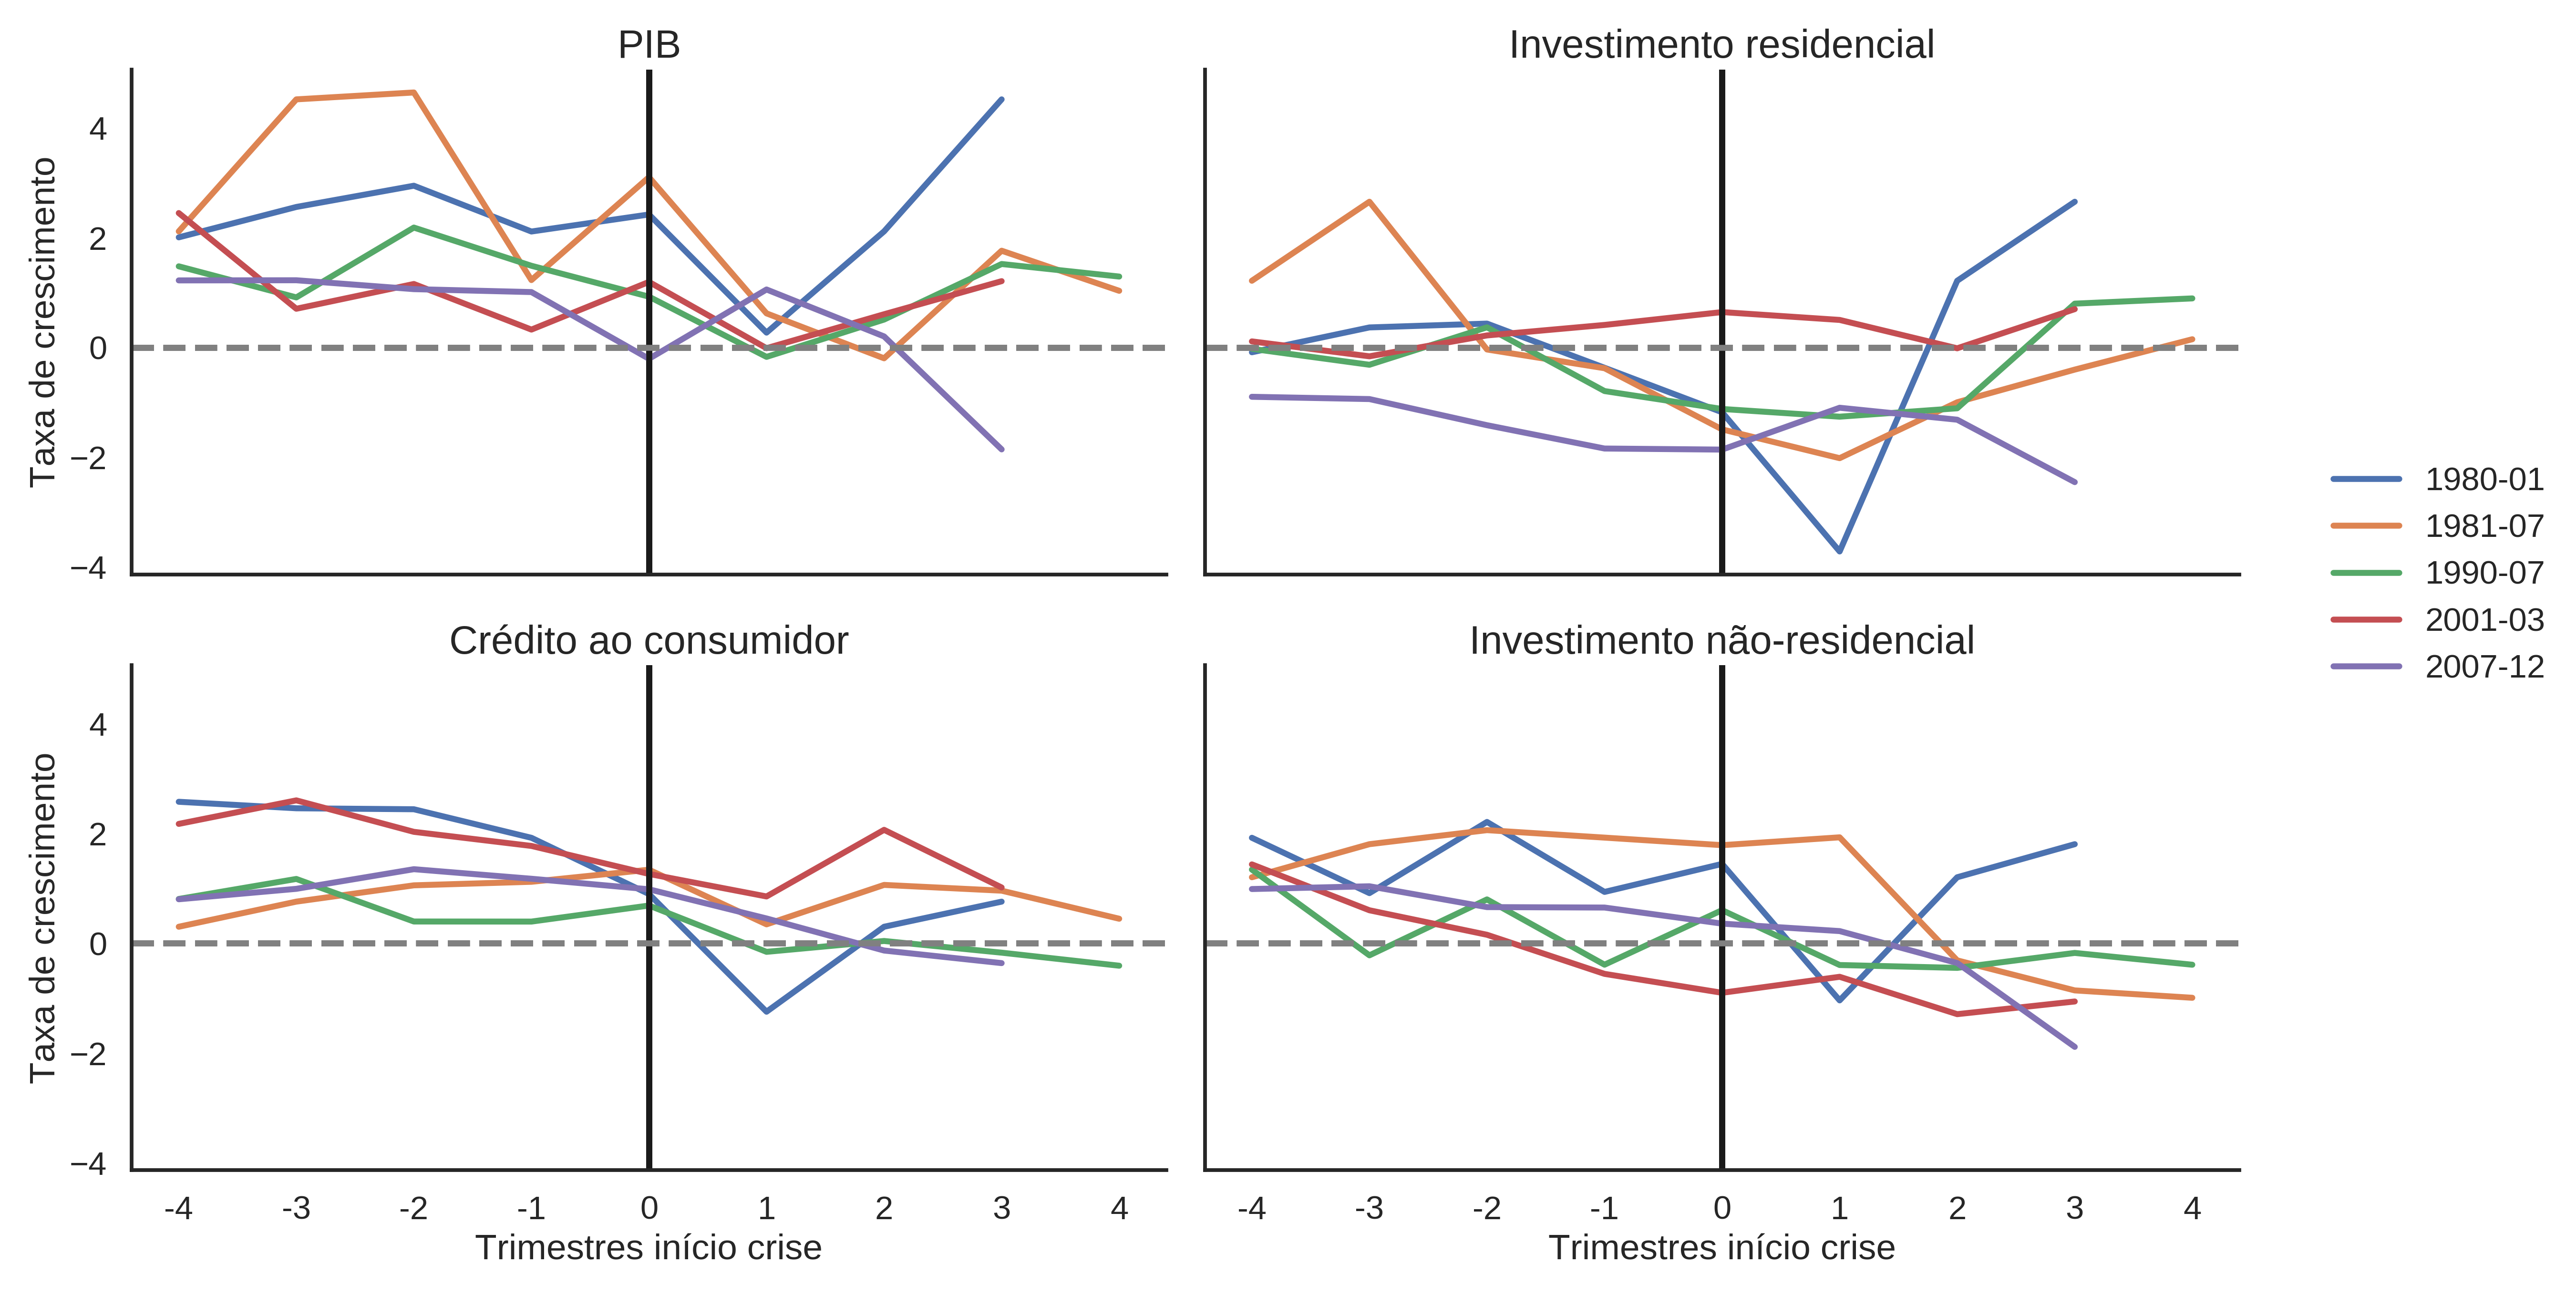
\includegraphics[width=\textwidth]{../../Dados/Fatos_Estilizados/figs/Centrado_Inicio_Norm.png}
	\caption*{\textbf{Fonte:} Elaboração própria}
\end{figure}

\begin{figure}[H]
	\centering
	\caption{Taxas de crescimento 4 trimestres antes e depois do início da  \textbf{recuperação} (normalizadas para manter a comparatibilidade)}
	\label{FigRecuperacaoNorm}
	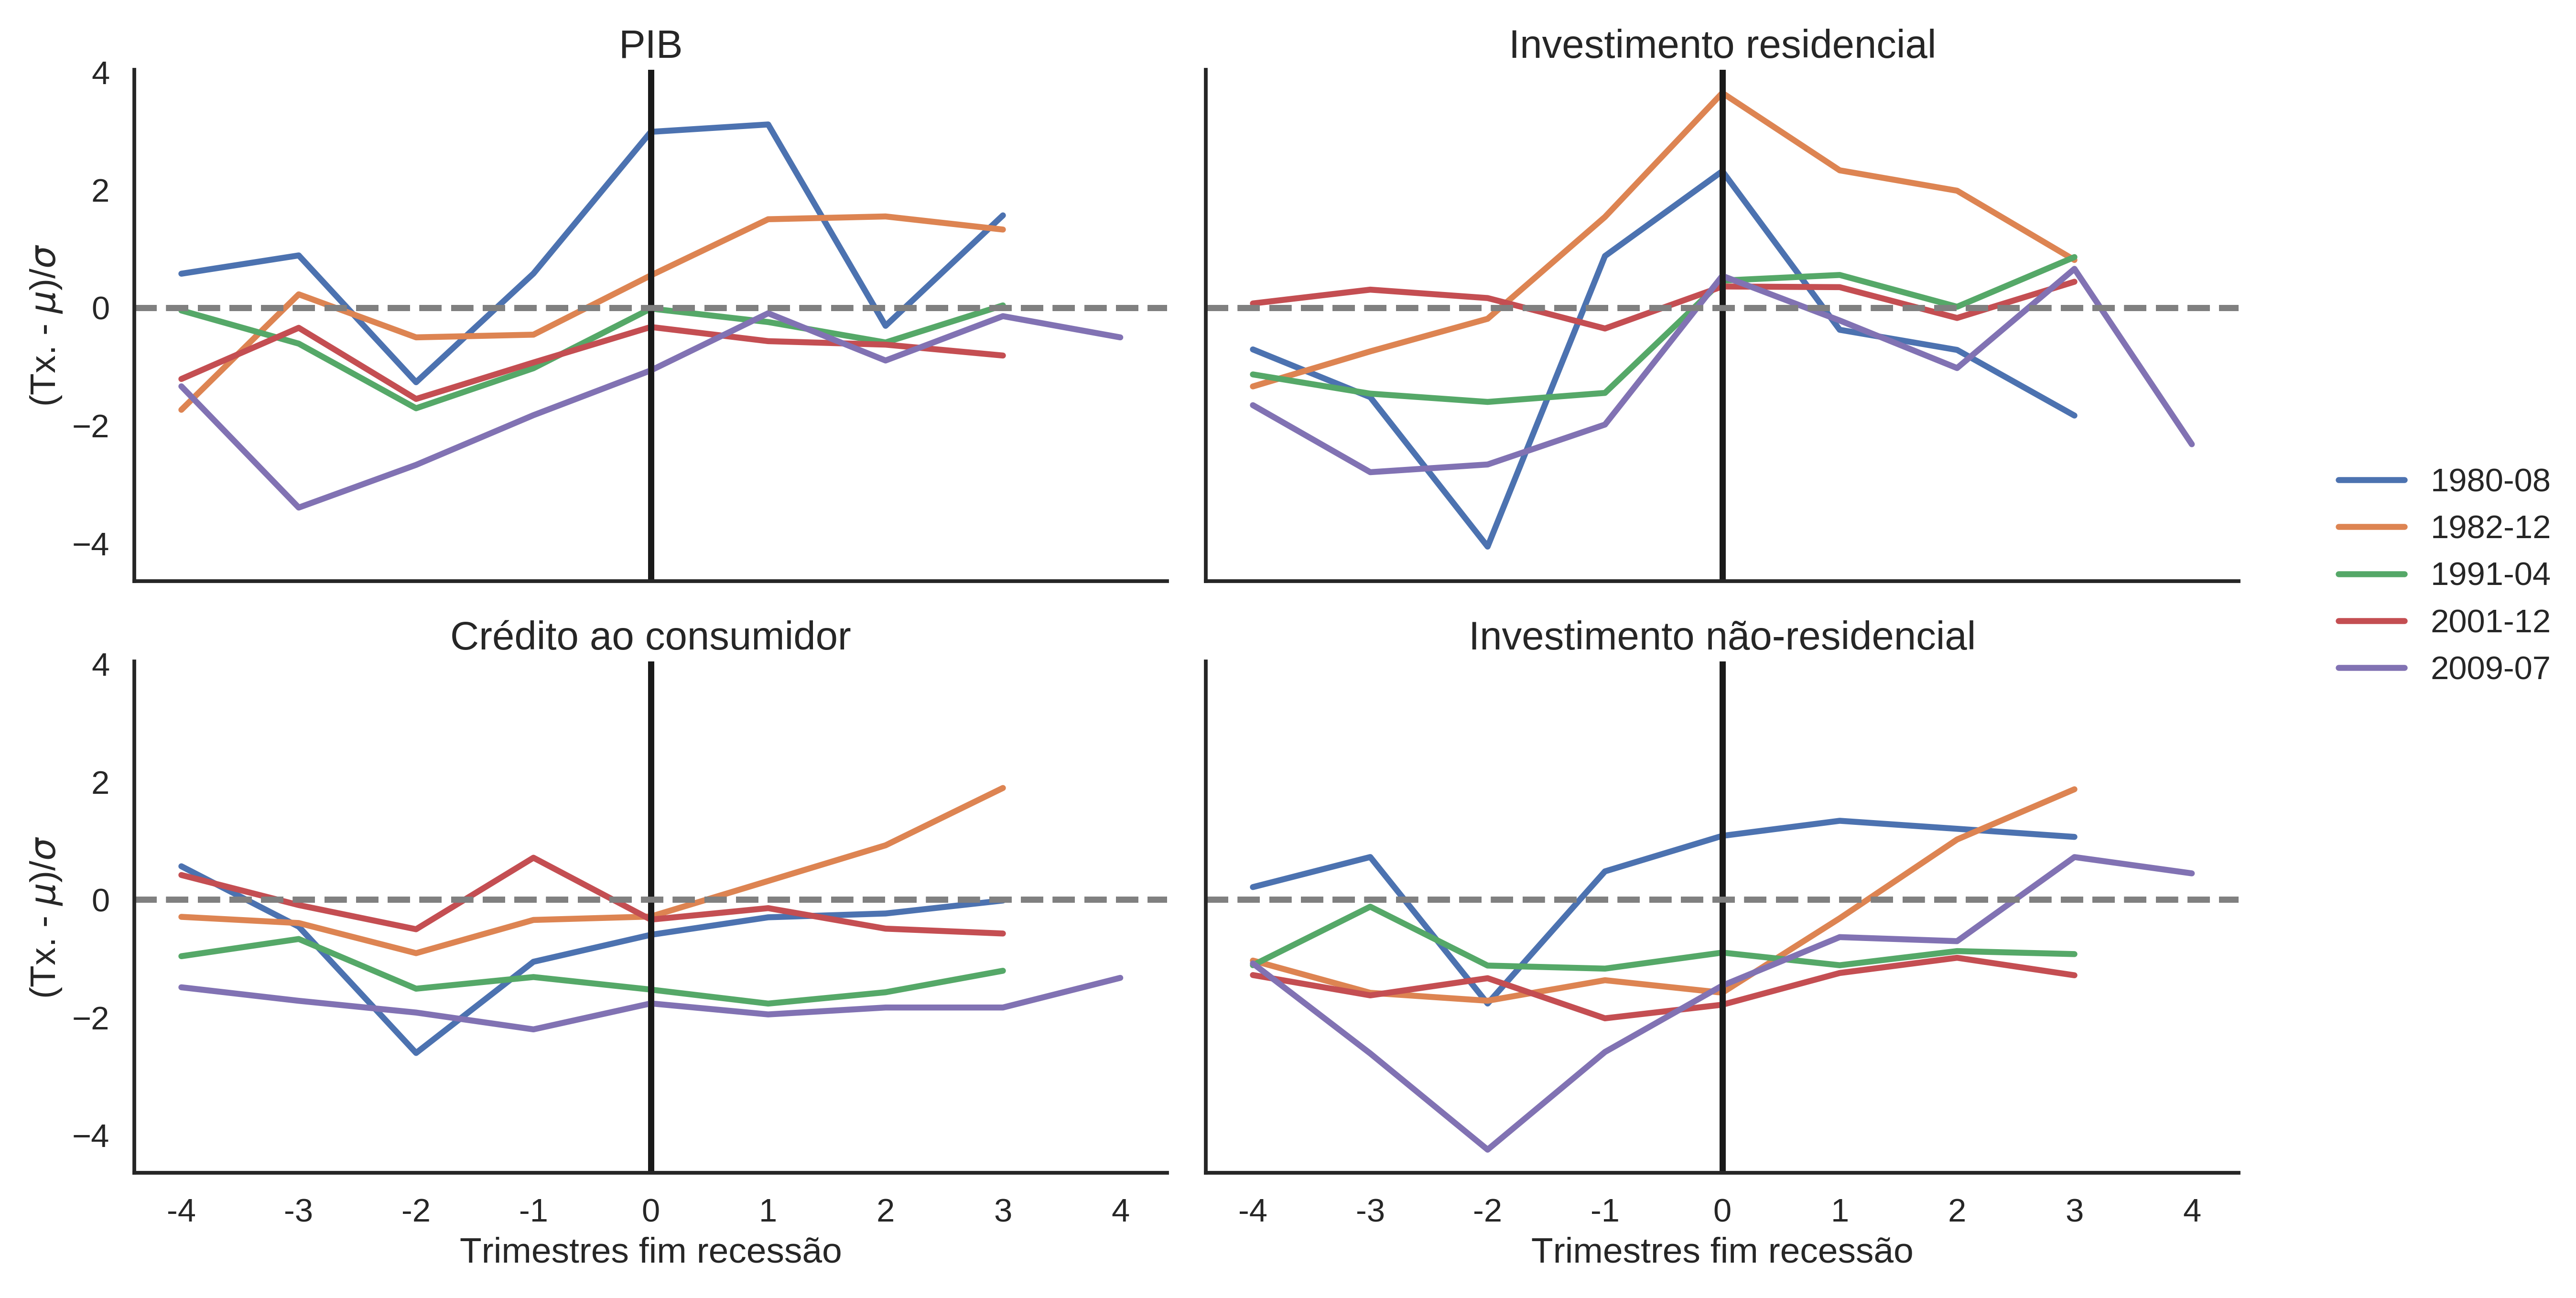
\includegraphics[width=\textwidth]{../../Dados/Fatos_Estilizados/figs/Centrado_Fim_Norm.png}
	\caption*{\textbf{Fonte:} Elaboração própria}
\end{figure}

%TODO Melhorar resolução do gráfico e linhas


Da discussão anterior, conclui-se que a caracterização do ciclo econômico como liderado pelo investimento residencial é bastante extensa uma vez que apresenta esta configuração ao menos desde o pós-guerra.
No entanto, ocorreram mudanças significantes --- que não anulam a relevância do investimento residencial --- na economia norte-americana no pós-década de 80 que precisam ser analisadas em maior detalhe.
Um primeiro elemento é a estagnação salarial e os respectivos efeitos sobre o endividamento das famílias na calda inferior da distribuição \cites{barba_rising_2009}{teixeira_uma_2011}. 
Este endividamento, no entanto, não foi destinado a uma ampliação desproporcional do consumo, mas sim para a preservação do consumo habitual das famílias
\cites{wolf_rising_2010}{cynamon_inequality_2013}.


\begin{figure}[H]
	\centering
	\caption{Distribuição pessoal da renda (percentis selecionados, jan/1980 = 100)}
	\label{FigDistPessoal}
	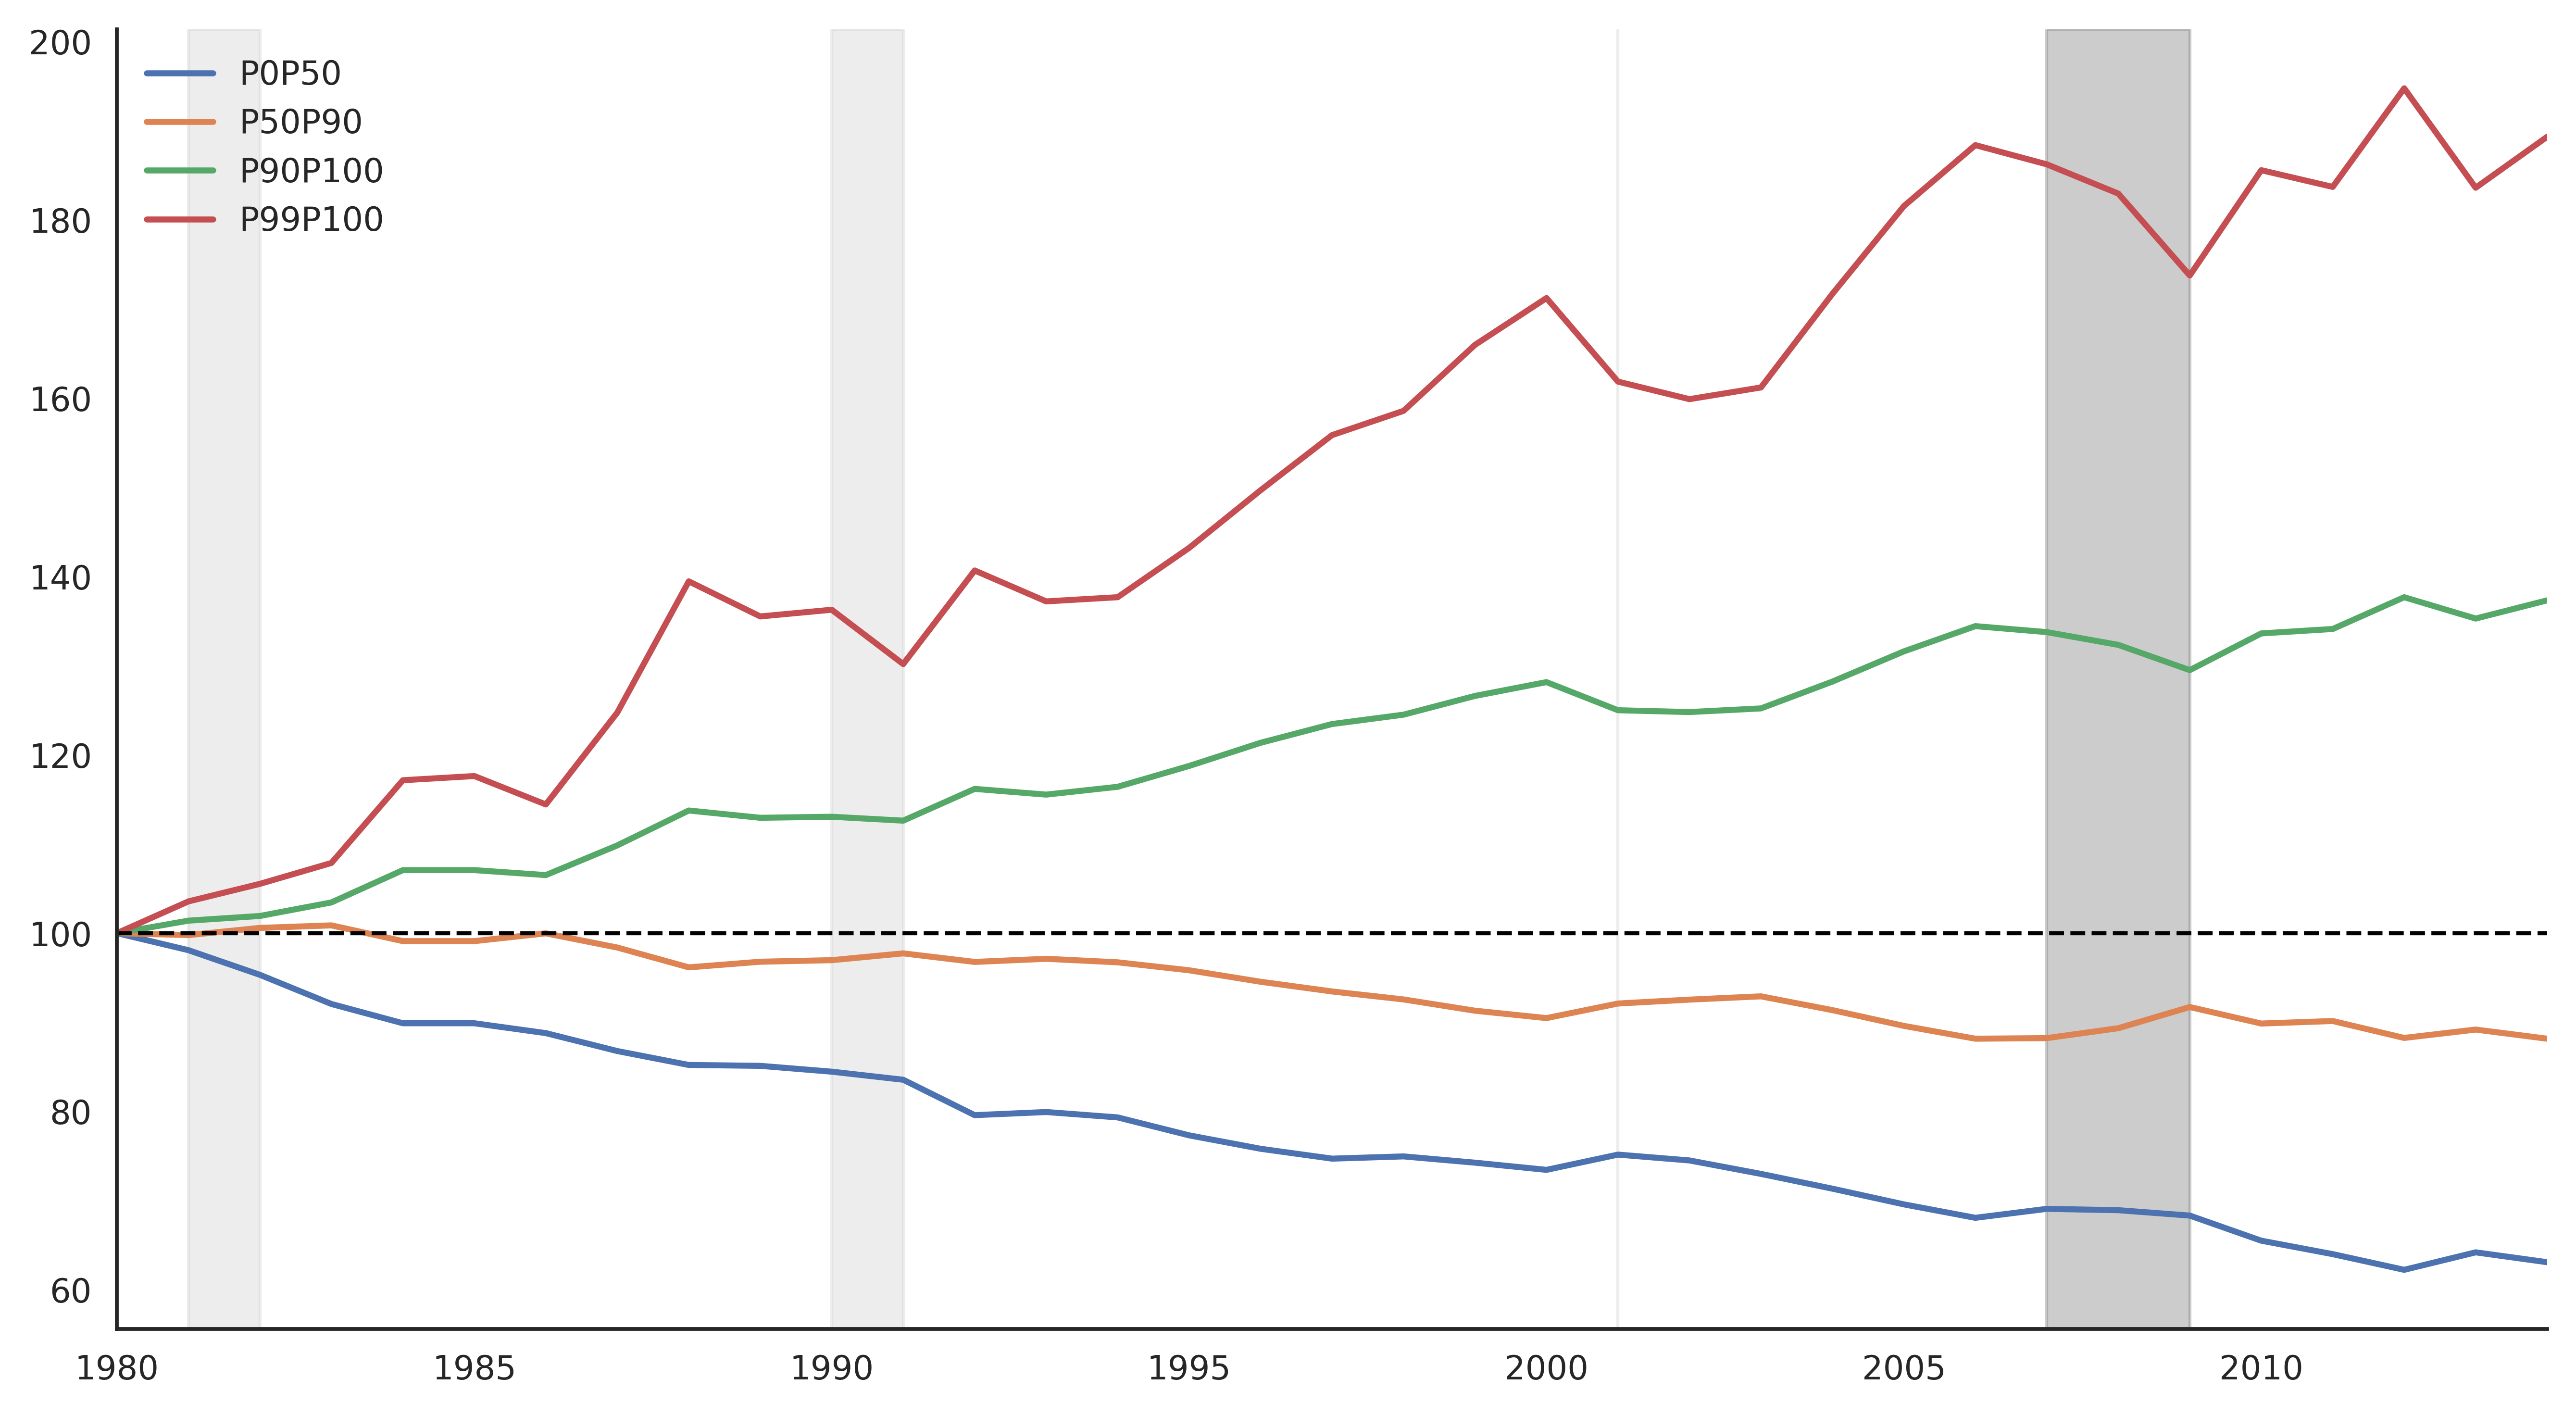
\includegraphics[width=\textwidth]{../../Dados/Fatos_Estilizados/figs/Dist_Pessoal.png}
	\caption*{\textbf{Fonte:} World Inequality Database (WID), elaboração própria}
\end{figure}


Estas mudanças distributivas tiveram impactos que vão além efeitos sobre a demanda agregada e se estendem para a recomposição de ativos (reais e financeiros) entre os estratos de riqueza.
Analisando a distribuição relativa dos ativos (gráfico \ref{FigDistAtivos}), destaca-se que os 50\% mais pobres ganharam participação relativa dos imóveis se comparado com 1979 até meados dos anos 90 ---  comportamento este espelhado pelos 1\% mais ricos. 
Em outras palavras, os imóveis passaram a compor uma parcela cada vez maior do portfólio de ativos deste estrato enquanto os ativos financeiros apresentaram uma tendência de queda persistente.
Enquanto a participação dos imóveis dentre os mais pobres foi crescente e oscilante ao longo do período, o mesmo não pode ser dito sobre os bens duráveis, indicando já mencionada tentativa manutenção do padrão de consumo frente a estagnação salarial.
Além disso, este gráfico também sugere que a demanda por imóveis por motivos especulativos foi iniciada pelo estrato dos 1\% mais ricos e acompanhada pelo subsequente aumento na demanda por imóveis --- não necessariamente especulativa --- dos 50\% mais pobres.


\begin{figure}[H]
	\centering
	\caption{Distribuição de ativos por percentil de riqueza (1989/07=1)}
	\label{FigDistAtivos}
	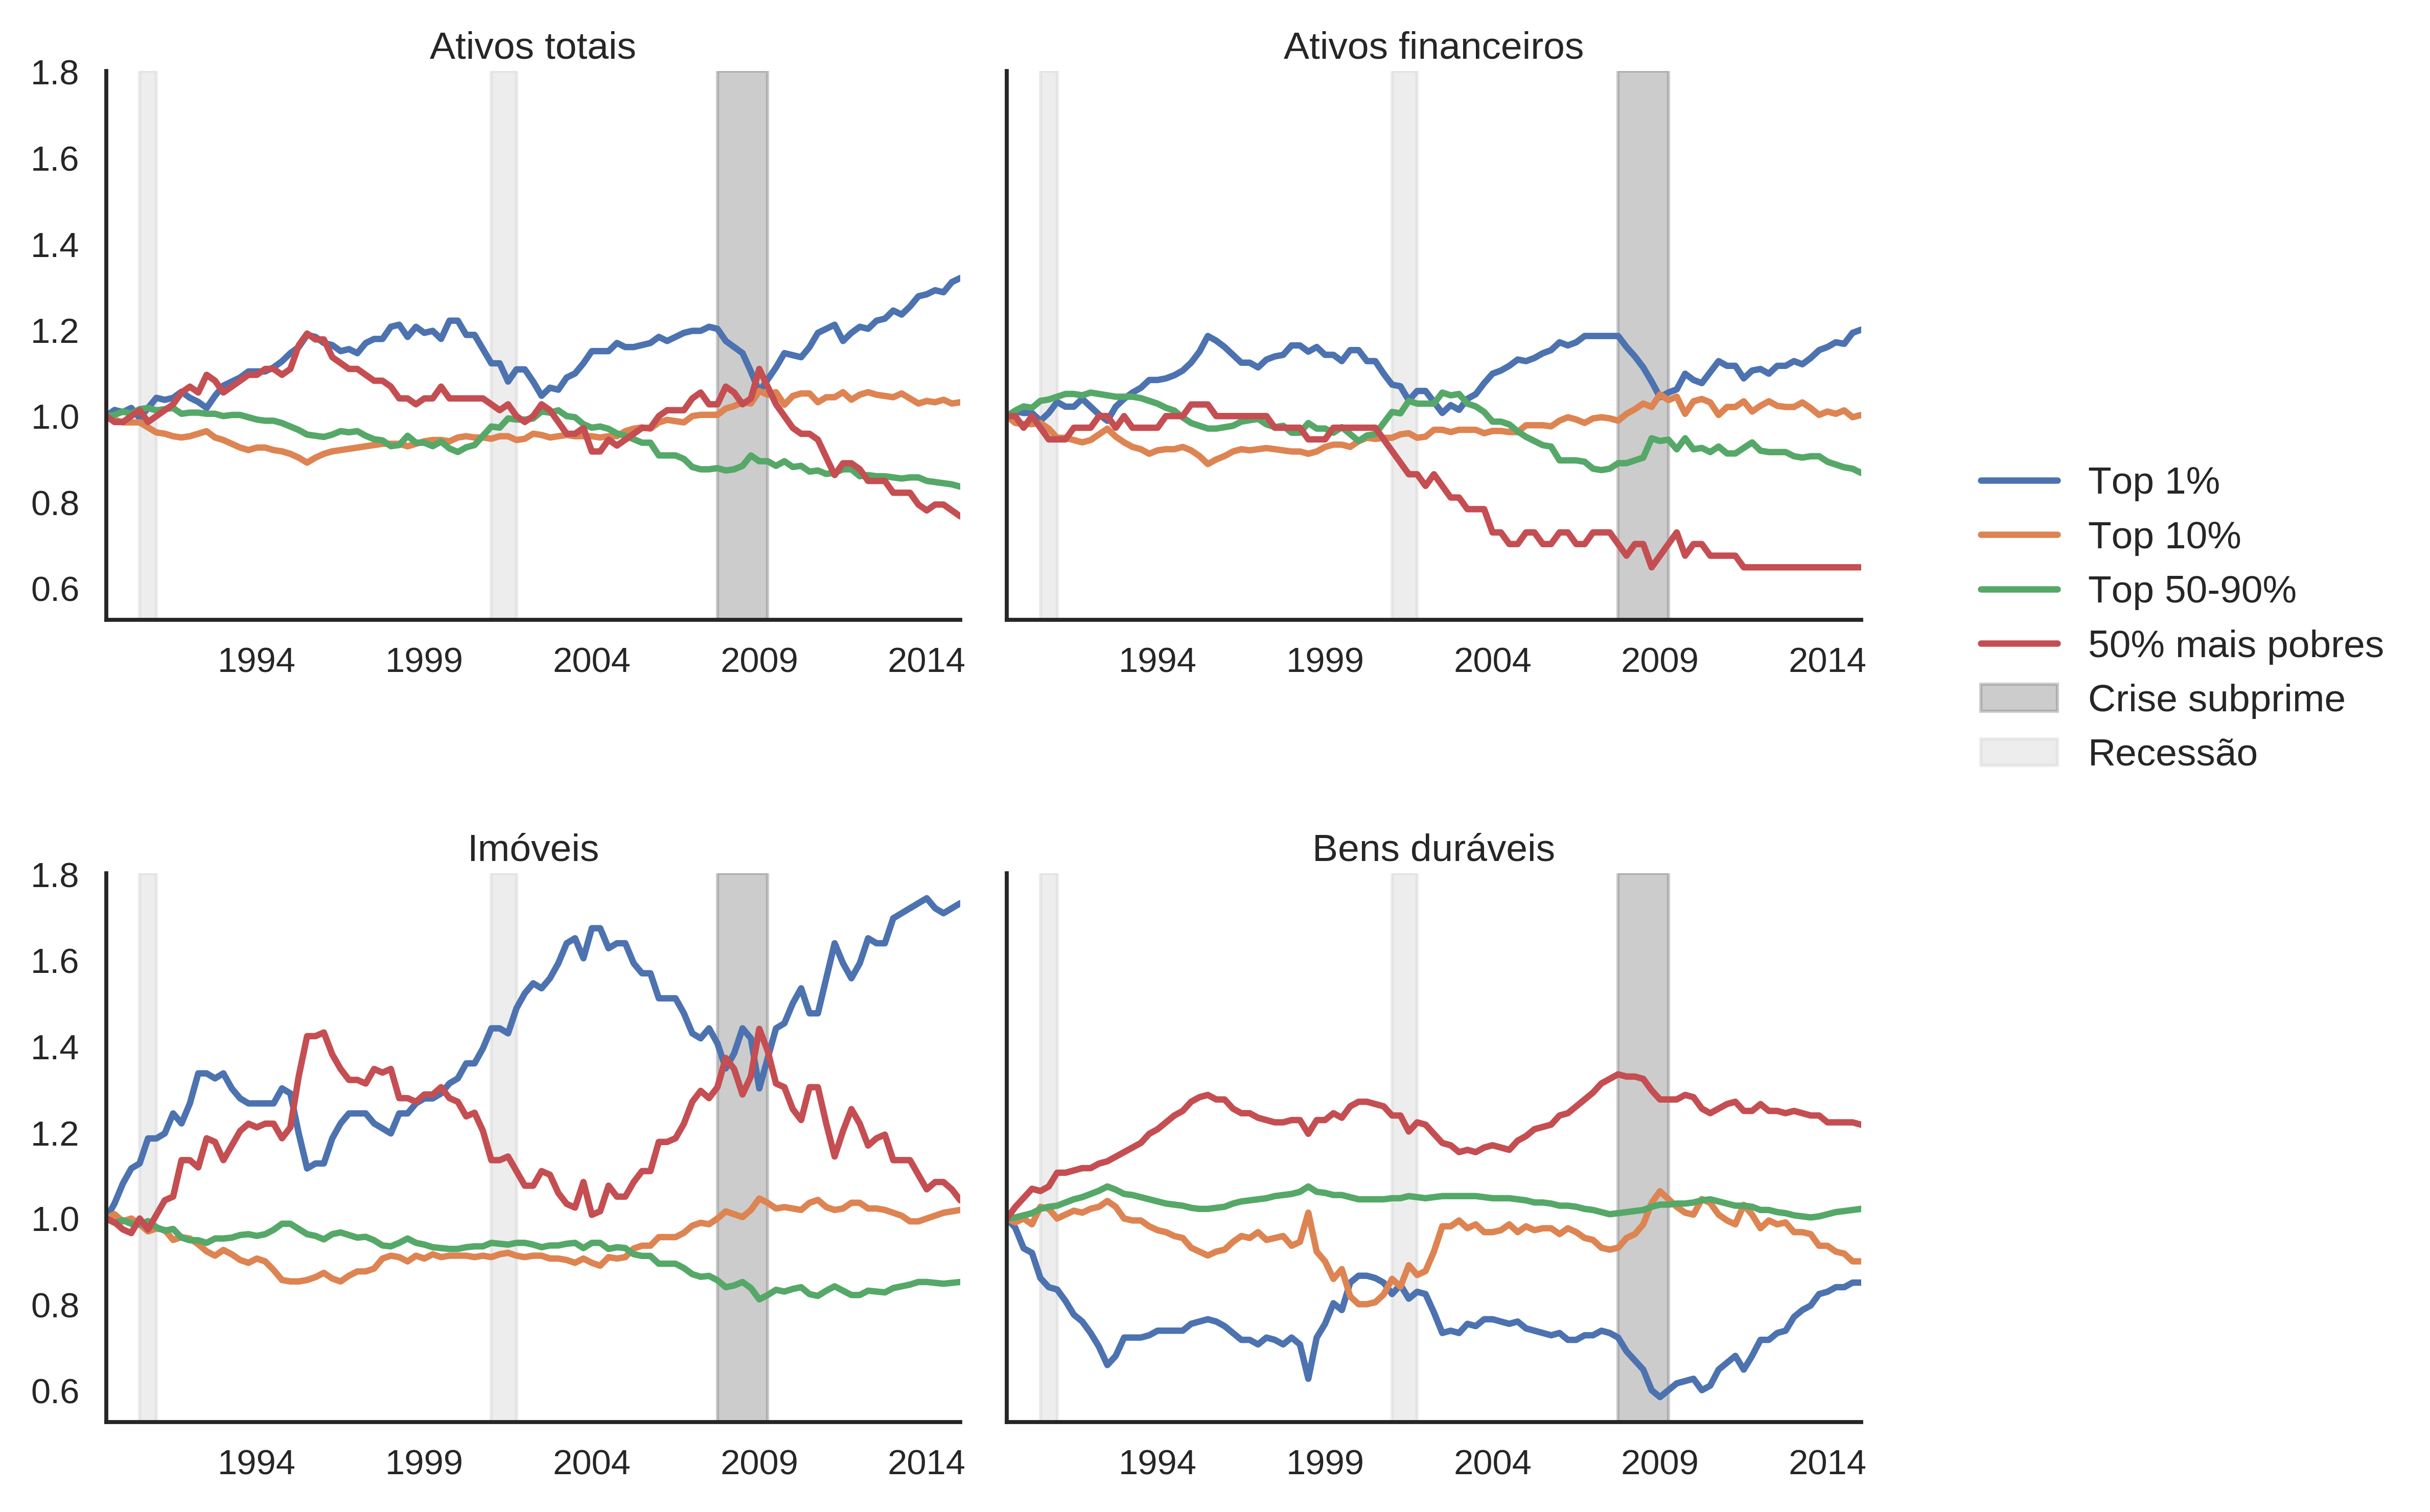
\includegraphics[width=\textwidth]{../../Dados/Fatos_Estilizados/figs/Distribuicao_Ativos.png}
	\caption*{\textbf{Fonte:} \textcite{us_census_bureau_characteristics_2017}, Elaboração própria}
\end{figure}

Os passivos (gráfico \ref{FigDistPassivos}), por sua vez, apresentam uma dinâmica semelhante entre si, ou seja, a participação nos empréstimos e nas hipotecas  é bastante similar ao longo do período analisado.
Argumenta-se aqui que tal resultado decorre da permissividade institucional americana.
De acordo com \textcite{teixeira_uma_2011}, os imóveis são uma das formas de riqueza mais comuns entre as famílias norte-americanas, servindo de colateral para tomada de crédito. A forma de ``realizar'' o ganho de capital com a bolha imobiliária que ocorreu no período, sem precisar liquidar os imóveis, era justamente ampliando o endividamento à medida que o colateral (\textit{i.e.} imóveis) aumentava de valor \cite{teixeira_crescimento_2015}. 


\begin{figure}[H]
	\centering
	\caption{Distribuição de passivos por percentil de riqueza (1989/07=1)}
	\label{FigDistPassivos}
	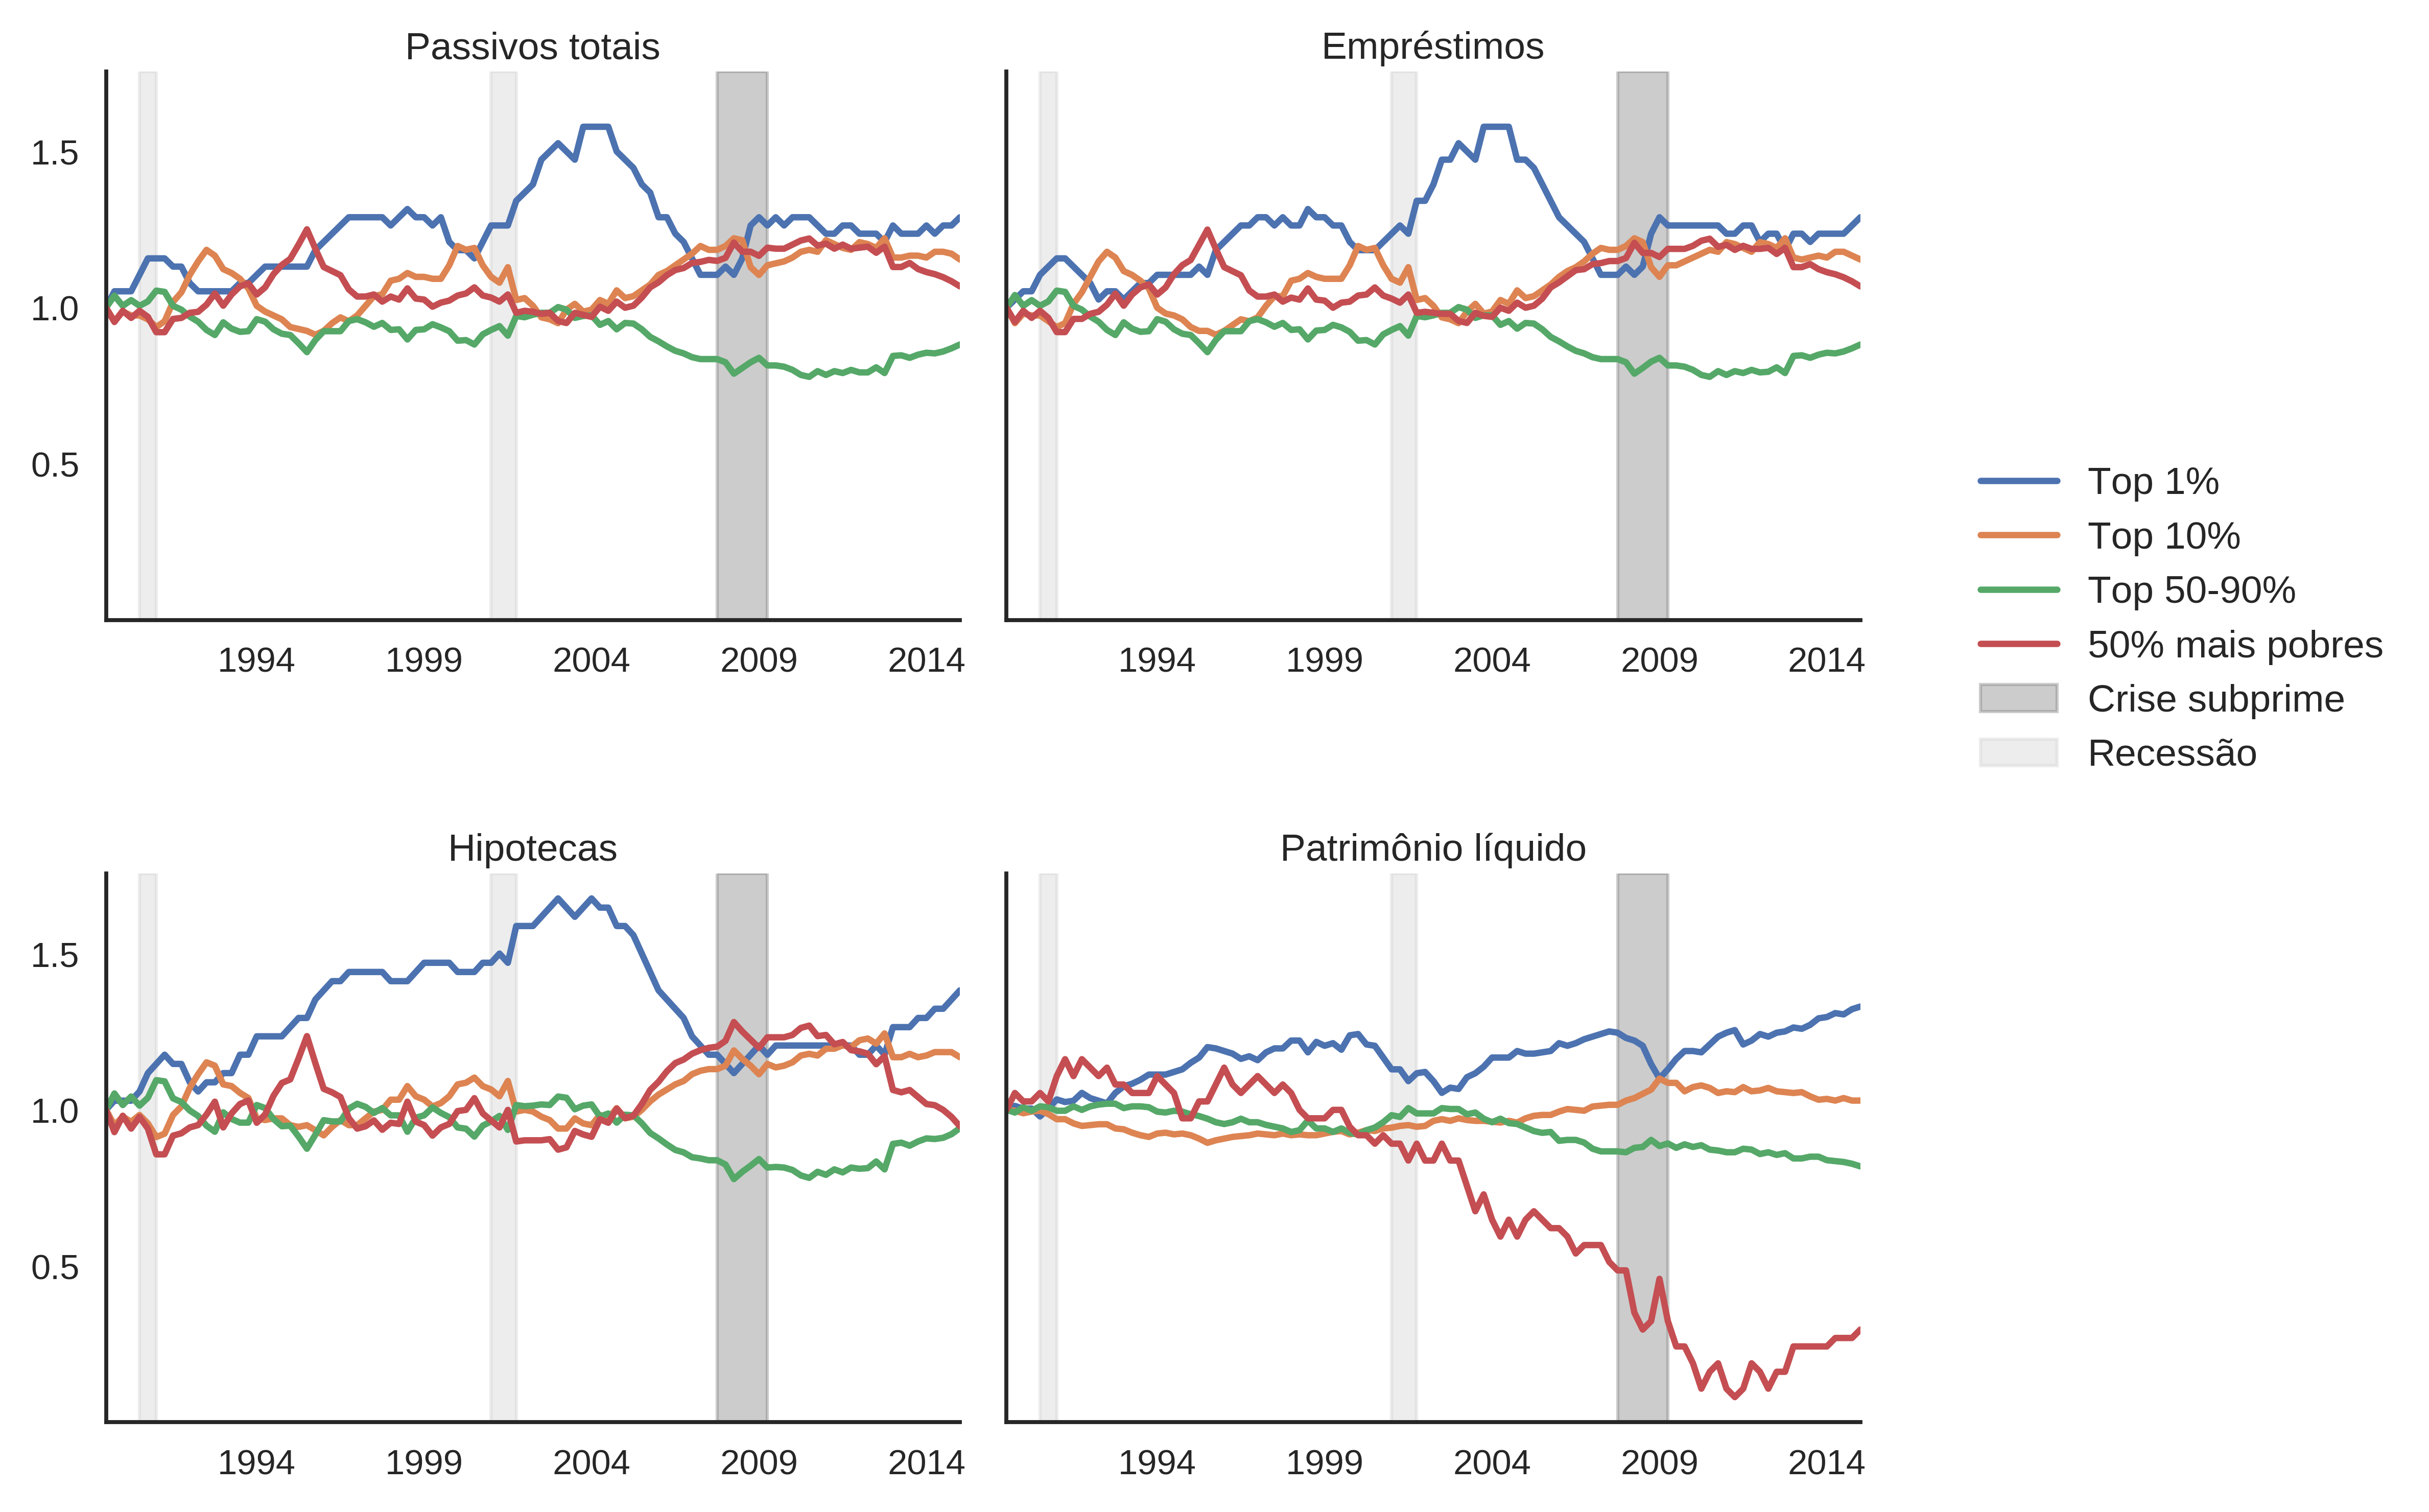
\includegraphics[width=\textwidth]{../../Dados/Fatos_Estilizados/figs/Distribuicao_Passivos.png}
	\caption*{\textbf{Fonte:} \textcite{us_census_bureau_characteristics_2017}, Elaboração própria}
\end{figure}


Como consequência, observa-se uma dinâmica gêmea (ver gráfico \ref{FigDividaPreco}) entre endividamento das famílias e preço dos imóveis que, por sua vez, permitia a ampliação do consumo --- sobretudo das famílias mais pobres --- mesmo com a estagnação salarial do período.
Tal especificidade institucional teve algumas implicações sobre a dinâmica macroeconômica que precisam ser melhor analisadas.
A primeira delas é o descolamento entre ativos e passivos no decorrer da crise financeira de 2008.
Esta separação decorre tanto do esgotamento da bolha dos imóveis (pós-2005) que fez com que os tais ativos desvalorizassem quanto da insensibilidade dos compromissos financeiros das famílias (\textit{i.e.} dívida) a queda do preço dos imóveis.
Em outras palavras, os imóveis (ativo) tem valor de mercado enquanto a dívida (passivo) tem um valor contratual sendo assim, o patrimônio líquido das famílias cai com o instaurar da crise.
A segunda implicação --- resultante da conjugação dos movimentos anteriores --- é a redução acentuada do patrimônio líquido das famílias mais pobres em termos absolutos e relativos (painel inferior direito do gráfico \ref{FigDistPassivos}).
Em resumo, a estagnação dos salários somada às inovações financeiras que permitiram ampliação do consumo por meio de ampliação no colateral das famílias associado a elevação do preços dos imóveis resultaram em uma substituição dos salários por dívida \cite{barba_rising_2009}.


\begin{figure}[H]
	\centering
	\caption{Dinâmica do endividamento das famílias e do preço dos imóveis (jan/2000=100)}
	\label{FigDividaPreco}
	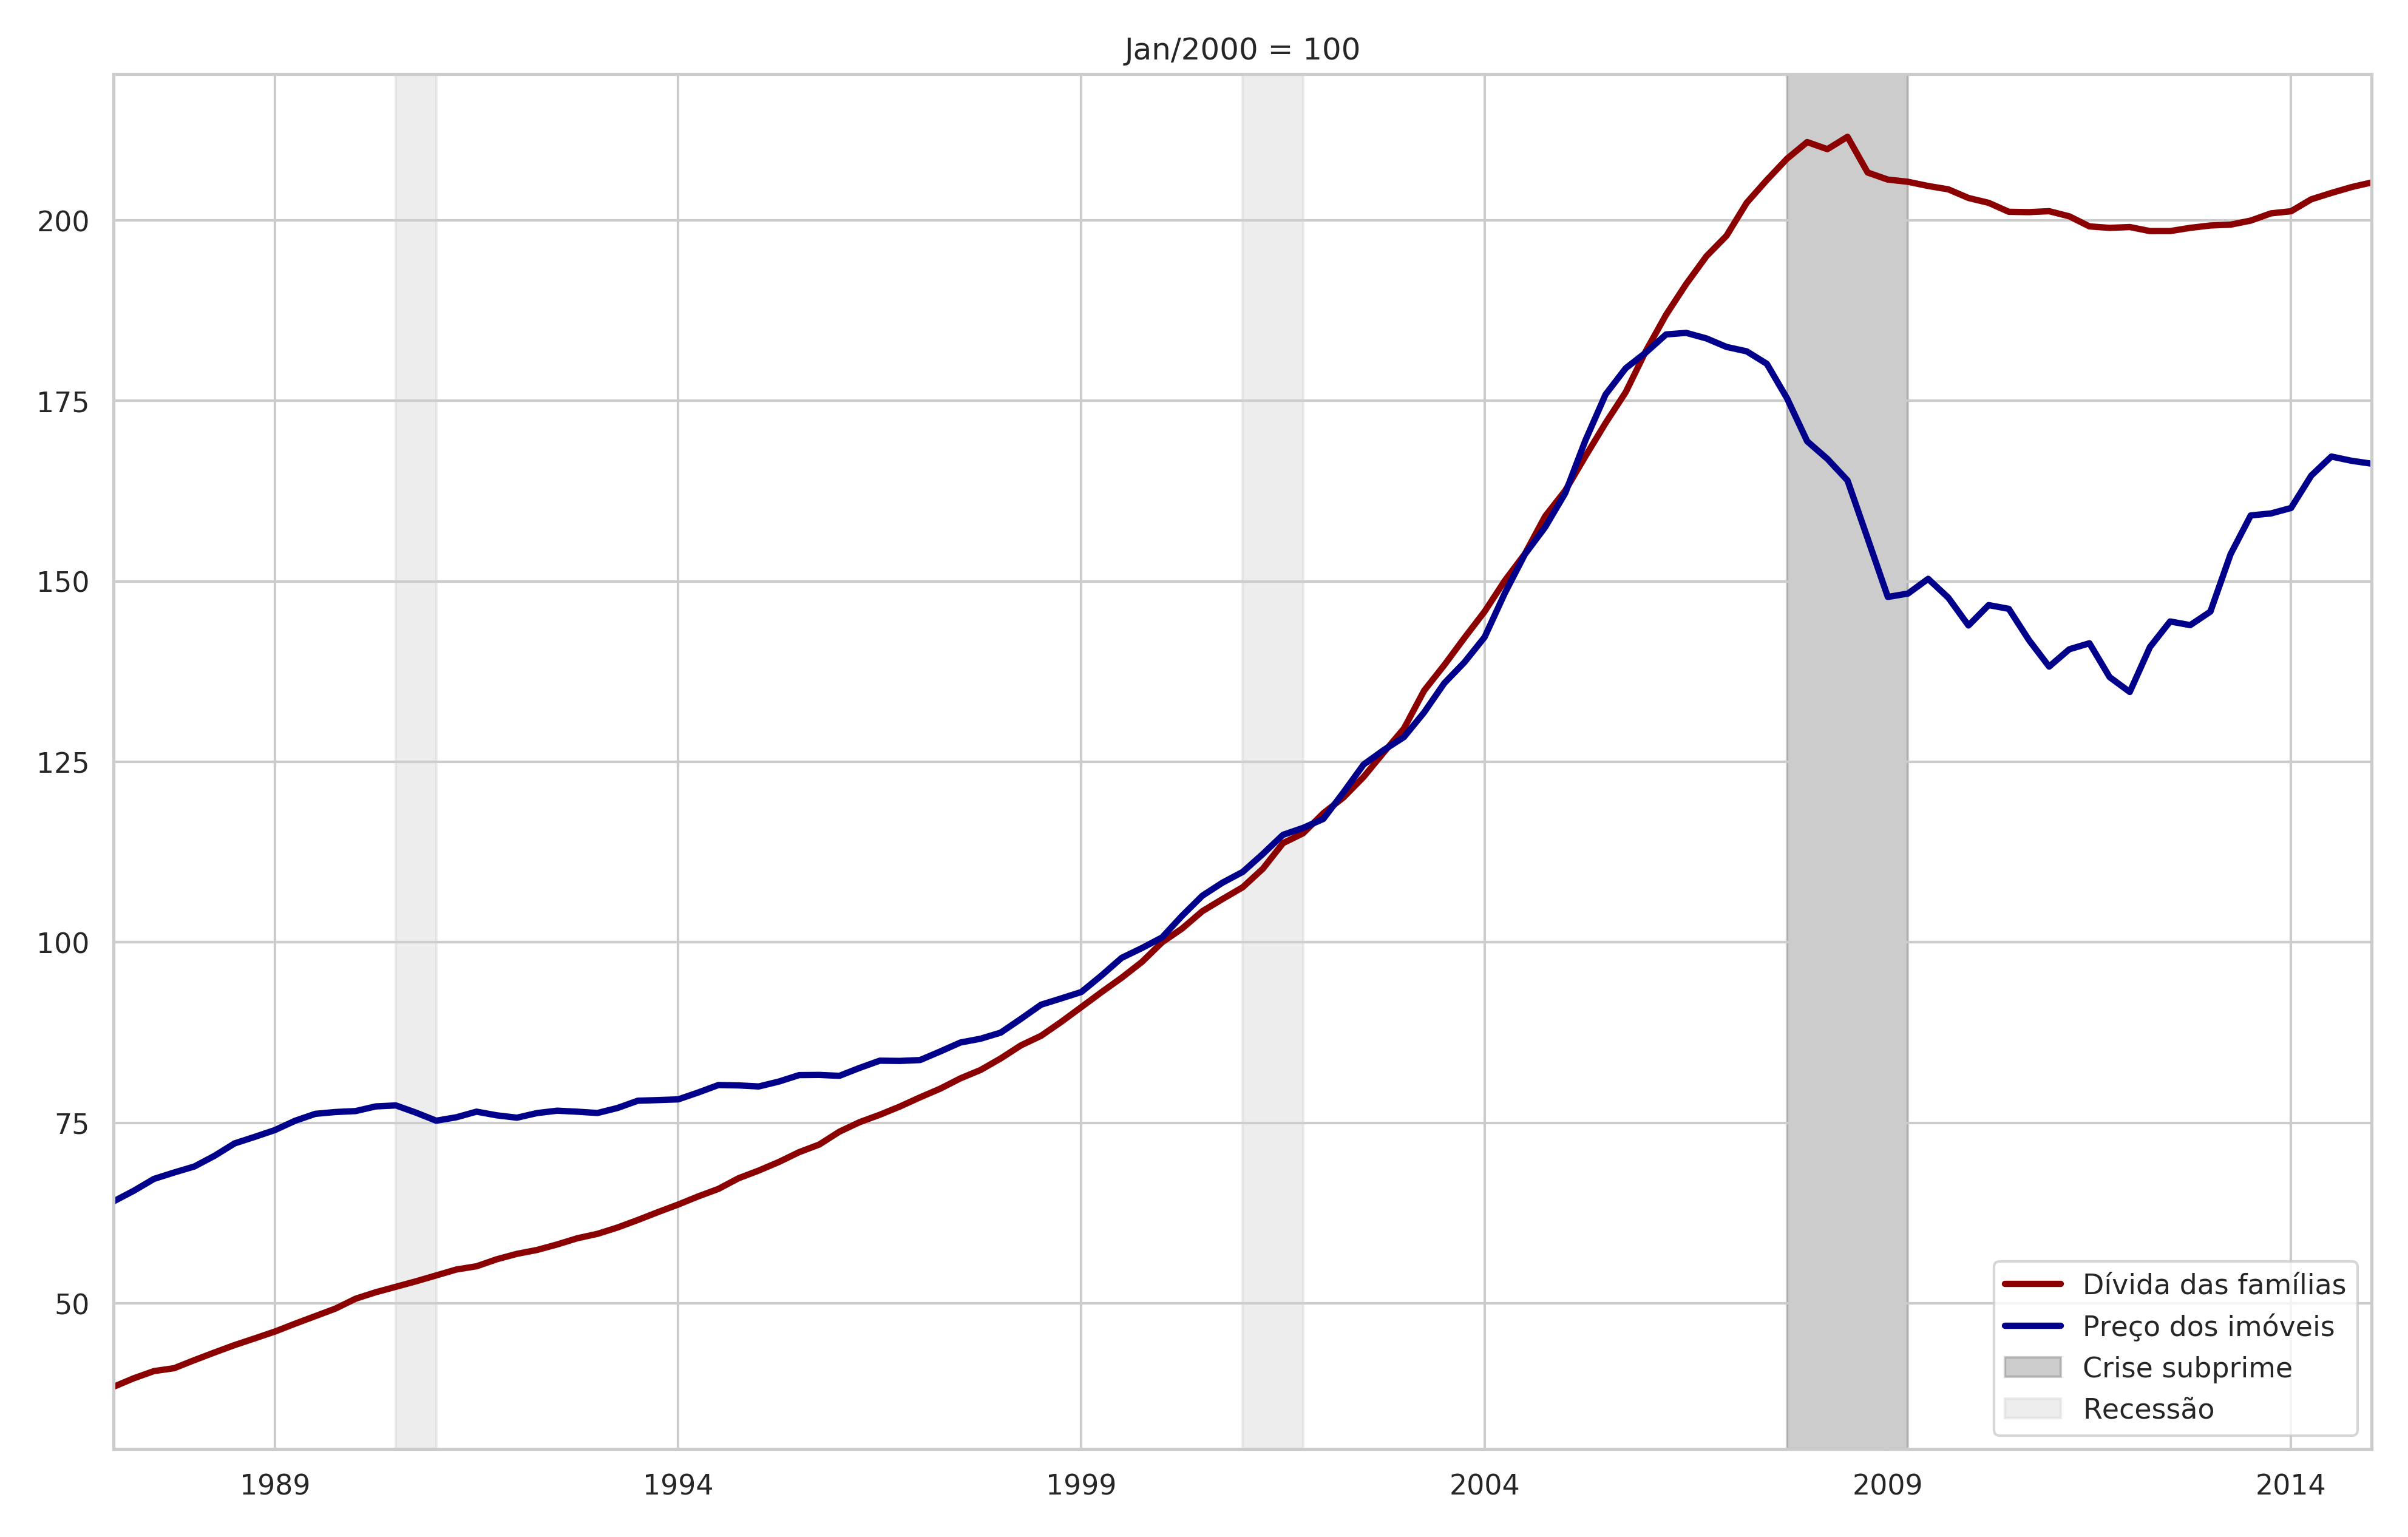
\includegraphics[width=\textwidth]{../../Dados/Fatos_Estilizados/figs/Divida_PrecoImoveis.png}
	\caption*{\textbf{Fonte:} U.S. Bureau of Economic Analisys, elaboração própria}
\end{figure}

\begin{figure}[H]
	\centering
	\caption{Comprometimento da renda das famílias com o pagamento de juros (jan/1980 = 100)}
	\label{FigServDiv}
	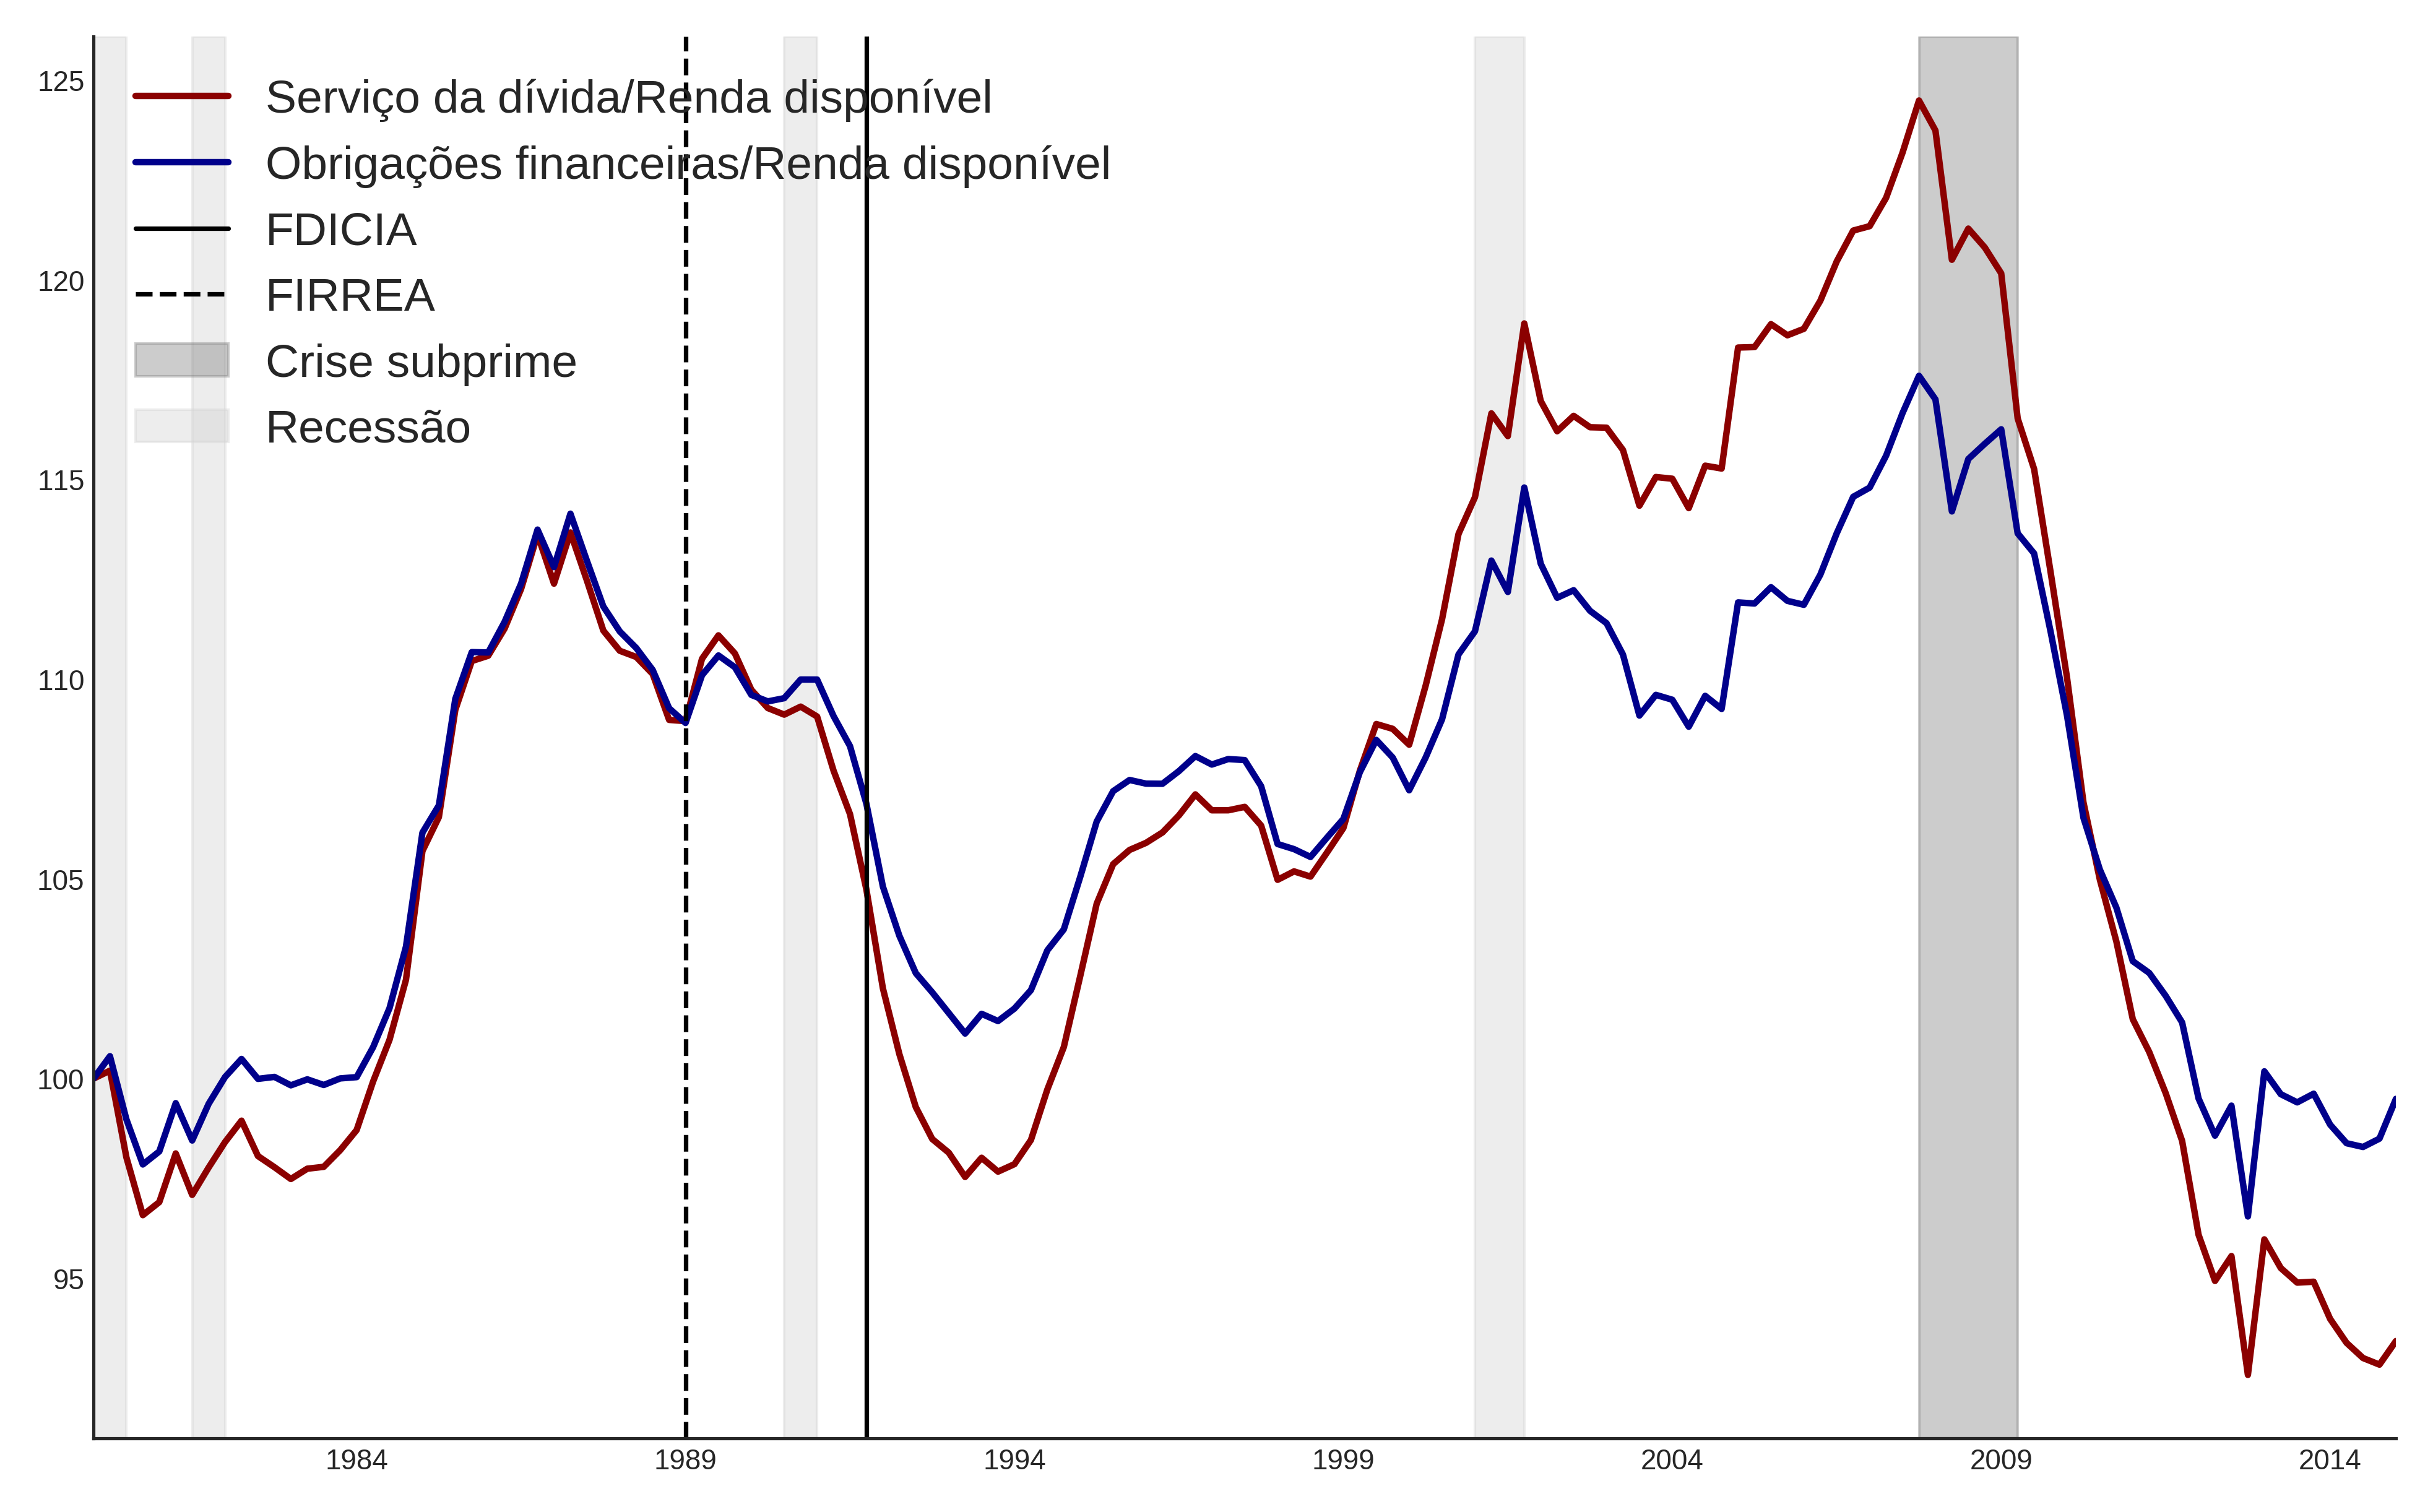
\includegraphics[width=\textwidth]{../../Dados/Fatos_Estilizados/figs/Serv_Divida.png}
	\caption*{\textbf{Fonte:} U.S. Bureau of Economic Analisys, elaboração própria}
\end{figure}


Existe também outra dimensão relevante que a literatura não dá a devida atenção: popularização dos imóveis primários\footnote{
	Em linhas gerais, um imóvel primário é aquele que o proprietário tem acesso regular e, no caso de possuir mais de um imóvel (secundário), é aquele que usufrui a maior parte do tempo ao longo do ano \cite{us_census_bureau_characteristics_2017}.
}.
A ampliação do acesso às residências pode ser visualizada no gráfico \ref{FigConcentracao} em que estão apresentadas as curvas de concentração\footnote{Em linhas gerais, curvas de concentração são elaboradas a partir da ordenação acumulada de duas variáveis (neste caso, riqueza e tipo de imóveis). Vale notar que a curva de Lorenz é um tipo específico de curva de concentração em que o eixo vertical apresenta a ordenação acumulada de uma única variável (normalmente renda).} de 1989 a 2010 por diferentes tipos de imóveis (primários e secundários).
%TODO Descrição dos imóveis primários e secundários
A partir destas curvas é possível avaliar quão concentrado é certo tipo de ativo comparando-o com a linha de perfeita igualdade\footnote{Quão mais acima e a esquerda da linha de perfeita igualdade menos concentrado/mais progressivo o ativo em questão está/é enquanto uma curva mais a direita e abaixo indica o oposto.
Neste caso, um ponto acima desta linha indica que o ativo em questão (neste caso, imóveis) é distribuído a favor dos estratos mais pobres da riqueza.
Além disso, a distribuição deste ativo contribuirá para a redução da desigualdade quanto mais inclinada for a curva de concentração na região dos mais pobres.
}.
Dito isso, uma breve inspeção deste gráfico revela que os anos que antecederam a crise dos \textit{subprime} foram caracterizados pela desconcentração dos imóveis primários, ou seja, estratos mais pobres da população passaram a deter uma parcela acumulada maior deste tipo de imóvel.
Uma vez que as residências primárias dizem respeito àquelas que são utilizadas para fins não necessariamente especulativos, verifica-se uma elevação generalizada da demanda por imóveis enquanto moradia e não enquanto ativos (ver também gráfico \ref{FigDistAtivos}).

%IMÓVEIS PRIMÁRIOS POR QUE SÃO ÚTEIS E SECUNDÁRIOS PELA ESPECULAÇÃO

O mesmo não pode ser dito sobre os imóveis secundários\footnote{
	De acordo com o \textit{Survey of Construction} \cite{us_census_bureau_characteristics_2017}, os imóveis secundários são aqueles em que: (i) os proprietários residem parte do ano apenas; (ii) está ao menos 50 milhas do imóvel primário e; (iii) não pode estar sujeito a um contrato de aluguel.
} cujo movimento de concentração/distribuição não é tão demarcado quanto no caso anterior.
Além disso, uma vez que este tipo de imóvel não é destinado ao uso regular de seu proprietário, uma maior distribuição deste ativo sugere uma ampliação da demanda por imóveis na expectativa de ganhos de capital\footnote{
	Como pontuado no corpo do texto, esta aumento da demanda por imóveis secundários \textit{pode} indicar --- mas não se restringe a --- aumento por motivos especulativos. Uma casa de férias, por exemplo, é um uso não-especulativo de uma residência secundária.
	De todo modo, argumenta-se que há relação entre imóveis secundários e especulação.
}.
Outro elemento que chama atenção é que as famílias mais ricas não são as principais detentoras deste tipo de riqueza uma vez que acumulam menos da metade destes imóveis ao longo do período analisado.



%TODO Citar Survey

\begin{figure}[H]
	\centering
	\caption{Curva de concentração por tipos de imóveis}
	\label{FigConcentracao}
	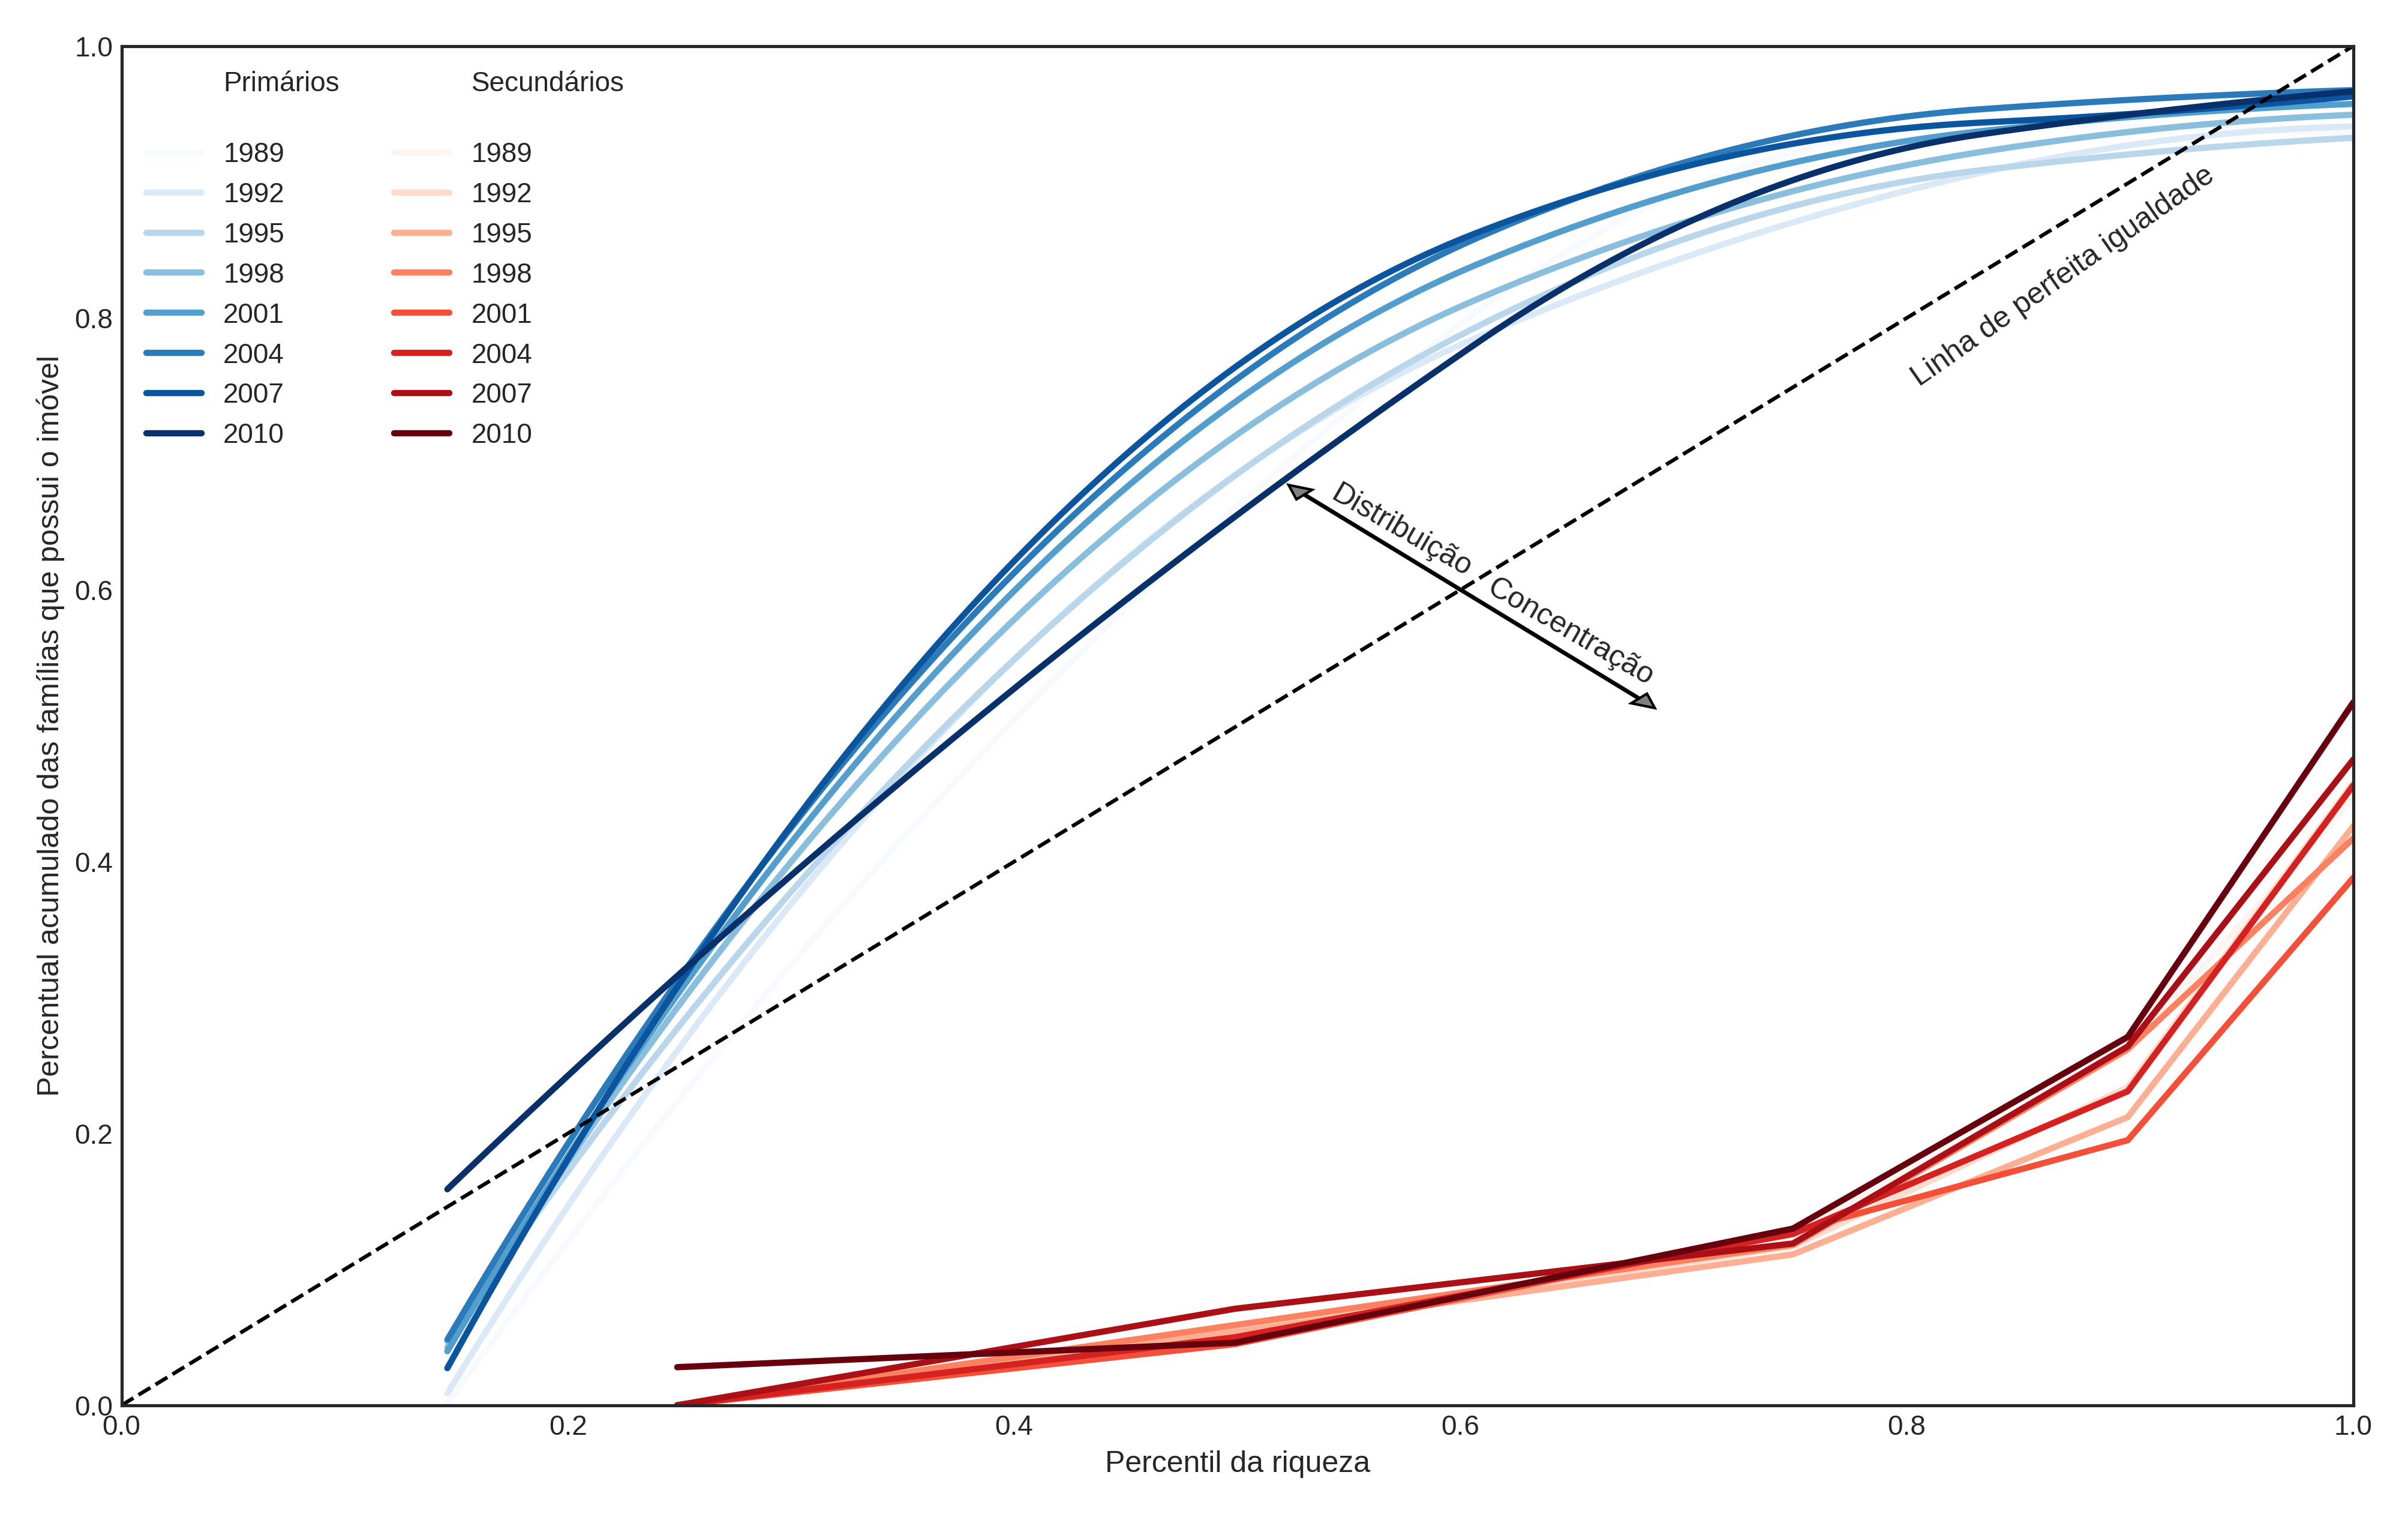
\includegraphics[width=\textwidth]{../../Dados/Fatos_Estilizados/figs/Concentracao_Imoveis.png}
	\caption*{\textbf{Fonte:} \textcite{us_census_bureau_characteristics_2017}, Elaboração própria}
\end{figure}
Por fim, partindo da hipótese apresentada no capítulo anterior (ver equação \ref{tx_Propria}) de que o investimento residencial possui um componente de longo prazo (popularização dos imóveis, por exemplo) e outro de médio prazo (especulação), argumenta-se que a relevância do aumento generalizado da participação dos imóveis entre os estratos de renda mais baixos decorre do maior grau de dependência de um número crescente de agentes econômicos da preservação das escalada dos preços dos imóveis.
Sendo assim, uma vez esgotada a bolha de ativos, os impactos são maiores que na ausência desta ``popularização residencial''.
%Isso somado a deterioração do patrimônio líquido das famílias mais pobres bem como maior comprometimento da renda disponível com o pagamento de juros (gráfico \ref{FigServDiv}) contribuiu para o delongamento da retomada desta crise mais recente.

%%%%%%%%%%%% RESUMO PARA OS CHOQUES
Em resumo, pontuou-se a relevância do investimento residencial para dinâmica macroeconômica.
Aliado a isso, outros fatos estilizados foram apresentados e que serão levados adiante no capítulo \ref{CapModelo}, são eles:
	(i) ampliação do consumo via a bolha imobiliária;
	(ii) popularização dos imóveis primários;
	(iii) redução da participação dos salários na renda e; principalmente 
	(iv) investimento residencial antecipa e determina a taxa de crescimento da economia.
Apresentados estes fatos estilizados, cabe a seção seguinte investigar como a literatura econométrica tem tratado o investimento residencial em termos macroeconômicos.

%Teixeira e a taxa própria
